%
% Simple template for generating drafts of papers and articles
%
\documentclass[12pt,]{article}
\usepackage{authblk}
\usepackage{fullpage}
\usepackage{amssymb,amsmath}
\usepackage[utf8x]{inputenc}
\usepackage[T1]{fontenc}
\usepackage{siunitx}
\usepackage[version=3]{mhchem}
\usepackage{bm}
\usepackage{multirow}

\usepackage{natbib}
\bibliographystyle{genetics}

% \pagestyle{empty} % if suppressing page numbers

% to add line numbers
\usepackage[left]{lineno}
\linenumbers

\usepackage{setspace}
\onehalfspacing

\usepackage[unicode=true]{hyperref}
\hypersetup{breaklinks=true,
            bookmarks=true,
            colorlinks=false,
            pdfborder={0 0 0}}
\urlstyle{same} % don't use a different (monospace) font for urls

\setcounter{secnumdepth}{5}

\usepackage{graphicx}
\graphicspath{{figures/}}
% Redefine \includegraphics so that, unless explicit options are
% given, the image width will not exceed the width or the height of the page.
% Images get their normal width if they fit onto the page, but
% are scaled down if they would overflow the margins.
\makeatletter
\def\ScaleWidthIfNeeded{%
 \ifdim\Gin@nat@width>\linewidth
    \linewidth
  \else
    \Gin@nat@width
  \fi
}
\def\ScaleHeightIfNeeded{%
  \ifdim\Gin@nat@height>0.9\textheight
    0.9\textheight
  \else
    \Gin@nat@width
  \fi
}
\makeatother
\setkeys{Gin}{width=\ScaleWidthIfNeeded,height=\ScaleHeightIfNeeded,keepaspectratio}%

\newcommand{\beginsupplement}{%
        \setcounter{table}{0}
        \renewcommand{\thetable}{S\arabic{table}}%
        \setcounter{figure}{0}
        \renewcommand{\thefigure}{S\arabic{figure}}%
        \setcounter{equation}{0}
        \renewcommand{\theequation}{S\arabic{equation}}
     }

%%%%%%%%%%%%%%%%%%%%%%%%%%%%%%%%%%%%%%%%%%%%%%%%%%%%%%%%%%%%%%%%%%%%%%%%%%%%%%

\title{\textbf{Detecting frequency-dependent selection through the effects of genotype similarity on fitness components}}
\author[1,2]{Yasuhiro Sato\thanks{Co-correspondence: yasuhiro.sato@uzh.ch}}
\affil[1]{Department of Evolutionary Biology and Environmental Studies, University of Zurich, Winterthurerstrasse 190, 8057 Zurich, Switzerland}
\affil[2]{Research Institute for Food and Agriculture, Ryukoku University, Yokotani 1-5, Seta Oe-cho, Otsu, Shiga 520-2194, Japan}
\author[3]{Yuma Takahashi}
\affil[3]{Graduate School of Science, Chiba University, Yayoi-cho 1-33, Inage-ku, Chiba 263-8522, Japan}
\author[1]{Chongmeng Xu}
\author[1,4]{Kentaro K. Shimizu\thanks{Co-correspondence: kentaro.shimizu@ieu.uzh.ch}}
\affil[4]{Kihara Institute for Biological Research, Yokohama City University, Maioka 641-12, Totsuka-ward, Yokohama 244-0813, Japan}

\date{\today}

%%%%%%%%%%%%%%%%%%%%%%%%%%%%%%%%%%%%%%%%%%%%%%%%%%%%%%%%%%%%%%%%%%%%%%%%%%%%%%

\begin{document}

\maketitle


\newpage
\section*{Abstract}
Frequency-dependent selection (FDS) drives an evolutionary regime that maintains or disrupts polymorphisms. Despite the increasing feasibility of genetic association studies of fitness components, there are few methods to uncover the loci underlying FDS. Based on a simplified model of pairwise genotype-genotype interactions, we propose a linear regression that can infer FDS from observed fitness. The key idea behind our method is the inclusion of genotype similarity as a pseudo-trait in the selection gradient analysis. Single-locus analysis of \textit{Arabidopsis} and damselfly data could detect known negative FDS on visible polymorphism that followed Mendelian inheritance with complete dominance. By extending the single-locus analysis to genome-wide association study (GWAS), our simulations show that the regression coefficient of the genotype similarity can distinguish negative or positive FDS without confounding other forms of balancing selection. Field GWAS of the branch number further revealed that negative FDS, rather than positive FDS, was enriched among the top-scoring single nucleotide polymorphisms (SNPs) in \textit{Arabidopsis thaliana}. These results illustrate the wide applicability of our method for FDS on both visible polymorphism and genome-wide SNPs. Our study provides an effective way of selection gradient analysis to understand the maintenance or loss of polymorphism. [193 up to 200 words for target journals] 

\medskip
\noindent
\textbf{Keywords:} Frequency-dependent selection, Genome-wide association study, Pairwise interaction model, Selection gradient analysis

\medskip
\noindent
\textbf{Running title:} Detecting frequency-dependent selection

\newpage

\section{Introduction}
Widespread polymorphism is a remarkable hallmark of the genomes of wild organisms. Balancing selection occurs when multiple alleles are maintained at a single locus through negative frequency-dependent selection (FDS), overdominance, and spatiotemporal variation in selection pressure \citep{hedrick2007balancing}. Among these mechanisms, negative FDS favors rare alleles over common alleles and consequently maintains multiple alleles at a locus. To date, negative FDS has been reported to act on various polymorphic traits, such as coloration \citep{gigord2001negative, takahashi2010negative, le2015evolutionary, nosil2018natural}, self-incompatibility \citep{llaurens2008does, joly2011migration, shimizu2015evolution}, and resistance to natural enemies \citep{antonovics1984experimental, brunet2000disease, sato2017herbivore}. Conversely, positive FDS favors common alleles over rare alleles and thus results in the loss of polymorphisms \citep{borer2010positive, garrido2016effect}.

High-throughput genotyping technology has now enabled us to reveal the genomic basis of ecologically important traits and/or fitness in wild organisms \citep{durham_genome-wide_2014, fisher_genetic_2016, nosil2018natural, exposito2019natural, tsuchimatsu2020adaptive}. Specifically, genome-wide single nucleotide polymorphism (SNP) data help depict fitness-genotype association across genomes. In genome-wide association studies (GWAS) and quantitative trait locus (QTL) mapping, many statistical genetic analyses are based on linear regressions of a trait on genotype values \citep{broman2009single, gondro2013genome}. If the target trait is a direct component of fitness, the regression coefficient of each locus would infer a selection gradient \citep{lande1983measurement} at a target locus. By repeating this selection gradient analysis for all SNPs, for example, a recent study has quantified directional selection on a genome of \textit{Arabidopsis thaliana} \citep{exposito2019natural}.

Despite its increasing appreciation, little is known about the applicability of genetic association studies for FDS. To develop a general model of FDS, population genetics theory has long modelled genotype’s fitness as a product between frequency of a focal genotype and its encounter frequency with the other genotypes, which is called pairwise interaction model \citep{schutz1969inter, cockerham1972frequency, asmussen_frequency-dependent_1990, trotter2007frequency, schneider_maximization_2008}. Originally developed for direct competition among neighboring plants \citep{schutz1969inter}, the pairwise interaction model has so far been introduced to direct competition and mating in insect populations \citep{alvarez2005models}. However, growing body of evidence suggests that FDS occurs not only through direct interactions but also through indirect interactions between genotypes \citep{antonovics1984experimental,gigord2001negative,takahashi2010negative,sato2017herbivore}. For example, natural enemies mediate negative FDS on plant resistance when they attack to undefended plants surrounding defended plants \citep{antonovics1984experimental, brunet2000disease, sato2017herbivore}. Male's mate choice also mediates negative FDS on female color polymorphism when male insects learn on different colors of female individuals \citep{van2001frequency,takahashi2010negative}. Furthermore, while the pairwise interaction model assumes random interactions among individuals within subpopulations e.g., mobile insects within split cages \citep{cosmidis1999rarer,fitzpatrick2007maintaining,takahashi2014evolution} or within split plant patches \citep{sato2017herbivore}, the local action of FDS among neighboring plants is also plausible in a continuous vegetation \citep{janzen1970herbivores, connell1971role, browne2016frequency} (also known as the Janzen-Connell effects). If the pairwise interaction model can be exchanged as a general regression model, selection gradient analysis of FDS would become feasible in diverse organisms under various spatial structures (Fig. \ref{fig1:scheme}a).

\begin{figure}[ht]
  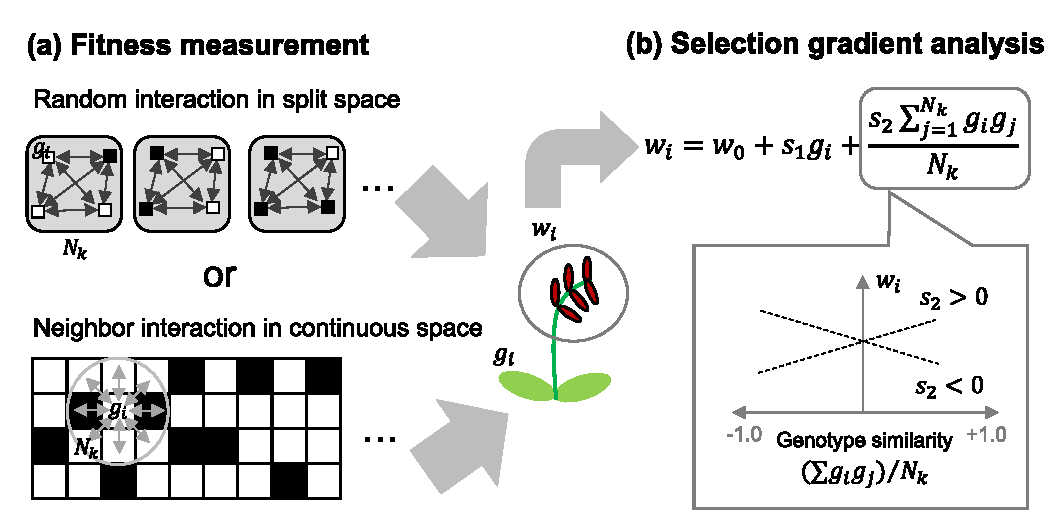
\includegraphics[width=0.8\linewidth]{scheme.pdf}
  \caption{Presumable scheme from the fitness measurement (a) to selection gradient analysis (b). (a) Individual fitness is observed as a consequence of pairwise interactions (two-way arrows) among individuals carrying different genotypes (black and white squares) within split subpopulations (upper gray squares: cf. the case of \textit{A. halleri} and \textit{I. elegans} in this study) or a continuous space (lower: cf. the case of \textit{A. thaliana}). (b) The selection gradient is then analyzed using a regression of the observed fitness $w_i$ on genotypes $g_i$. The second term in the equation is the same as Equation (\ref{eq:1}) in the main text and indicates how the second selection coefficient $s_2$ represents the effects of genotype similarity between the genotypes $g_i$ and $g_j$.
}
  \label{fig1:scheme}
\end{figure}

Previously, we proposed regression models that incorporated neighbor genotype similarity into genetic association studies \citep{sato2019neighbor, sato2020neighbor}. This idea was inspired by a model of ferromagnetism, which is widely known as the Ising model \citep{cipra1987introduction}. The pairwise physical interaction between two magnets to attract or repel each other may provide evolutionary insights into the effects of genetic interactions on spatiotemporal patterns and fitness consequences \citep{sato2019neighbor}. If two genotypes profit from their similarity, these positive interactions force similar genotypes to be clustered within the local space. If two genotypes profit from their dissimilarity, these negative interactions force dissimilar genotypes to be mixed across a space. Such a forward problem of the Ising model has been subject to genetic algorithms that mimic biological evolution \citep{anderson1991two, prugel1997dynamics}, because population optima are achieved through a series of updates on individual fitness. In contrast, an inverse problem of the Ising model poses how to estimate the coefficient of physical interactions from individual energy that is analogous to individual fitness. These analogies between the Ising model and biological evolution led us to hypothesize that the direction and strength of pairwise genetic interactions could be estimated by incorporating genotype similarity as a pseudo-trait into selection gradient analyses (Fig. \ref{fig1:scheme}b).

The purpose of this study is to develop an effective selection analysis that infers FDS based on observed fitness. Specifically, we investigated whether the Ising-based model of pairwise genetic interaction (i) can correctly detect known FDS by a single-locus analysis of visible polymorphic traits and (ii) screen FDS-associated polymorphisms from genome-wide SNPs. To accomplish these objectives, we first developed and applied the single-locus analysis to two examples under the split setting (Fig. \ref{fig1:scheme}a upper), including herbivore-mediated negative FDS on the trichome dimorphism of a wild herb \textit{Arabidopsis halleri} \citep{sato2017herbivore} and male-mediated negative FDS on the female color polymorphism of a damselfly \textit{Ischnura elegans} \citep{takahashi2014evolution}. The fact that trait expression of the trichome dimorphism and female color polymorphism both followed Mendelian inheritance with complete dominance \citep{shimizu2002ecology,sanchez2005hybridization,kawagoe2011coexistence} allowed us to substitute phenotype frequencies for genotype frequencies of the heterozygote and dominant homozygote. Extending the single-locus analysis to GWAS simulation, we then examined whether our method can detect simulated FDS from a number of genome-wide SNPs. Distinct population structures were assumed in this GWAS simulation: The split setting exemplified mobile animals in split cages with variable morph frequencies \citep{takahashi2014evolution} or plants in split plots \citep{sato2017herbivore}, where individuals are expected to interact uniformly within the cage or plot (Fig. \ref{fig1:scheme}a upper). In contrast, the continuous setting exemplified the Janzen-Connell effects \citep{janzen1970herbivores, connell1971role} in a forest or grassland, in which sessile organisms interact only with their neighbors and FDS is restricted to local areas (Fig. \ref{fig1:scheme}a lower). The extended GWAS method was finally applied for the branch number data on \textit{A. thaliana} accessions in order to screen polymorphisms associated with FDS under the continuous setting (Fig. \ref{fig1:scheme}a lower). The sort of theoretical and empirical analyses will show us the usage of our method for both visible polymorphic traits and genome-wide SNP data.


\section{Methods}

\subsection{Model development}
We developed a statistical method linking FDS, the Ising model, and a pairwise interaction model. First, we modeled pairwise interactions based on the forward problem of the Ising model. Then, we proposed a linear regression as an inverse problem of the Ising model. Finally, we examined fitness functions in a panmictic population to show how regression coefficients infer negative or positive FDS.

\subsubsection{Pairwise interactions based on the Ising model}
To model pairwise interactions between genotypes, we focused on the Ising model of ferromagnetics. Let us assume that diploid organisms interact within panmictic subpopulations and produce their offspring based on the realized fitness (Fig. \ref{fig1:scheme}a upper). We assume that a subpopulation $k$ belongs to the meta-population $K$ as $k \in K$, where two individuals $i$ and $j$ belong to subpopulation $k$ such that $i,j \in k$. We further assumed that individuals $i$ and $j$ had two alleles at a locus, with the ancestral allele A dominant over the derived allele a, where the genotype values were encoded as $g_{i(j)} \in$ \{AA, Aa, aa\} $=$ \{+1, +1, -1\}. This dominant encoding represented well-reported cases in which FDS often acts on a trait exhibiting dimorphism with complete dominance \citep[e.g.,][]{takahashi2010negative,sato2017herbivore}. By incorporating the genotype similarity between $i$ and $j$, we designated fitness $w$ for individual $i$ as:

\begin{equation}
w_i = w_0 + s_1 g_i + \frac{s_2}{N_k}\sum^{N_{k}}_{j=1}{g_ig_j}\label{eq:1}
\end{equation}
\noindent
where $w_0$ indicates the base fitness; $s_1$ and $s_2$ indicate the selection coefficients for self-genotype effects and genotype similarity, respectively; and $N_k$ indicates the total number of individuals within subpopulation $k$. The genotype similarity $\sum^{N_{k}}_{j=1}{g_ig_j}$ represents the similarity (or difference) of the genotype composition of the subpopulation from the individual $i$. If two individuals share the \textit{same} genotype values, $g_ig_j = (+1)\times(+1) = (-1)\times(-1) = +1$. If two individuals have \textit{different} genotype values, $g_ig_j = (-1)\times(+1) = (+1)\times(-1) = -1$. Thus, the within-population genotype similarity $(\sum^{N_{k}}_{j=1}{g_ig_j})/N_k$ ranges from -1.0 (perfect dissimilarity) to +1.0 (perfect similarity; Fig. \ref{fig1:scheme}b) as scaled by the total number of interacting individuals within the subpopulation $N_k$. In addition, we could also assume an additive expression for a trait responsible for FDS as $g_{i(j)} \in$ \{AA, Aa, aa\} $=$ \{+1, 0, -1\}, where the products involving heterozygotes were considered $0 \times 0 = 0$ (neither similar nor dissimilar). This additive encoding enabled us to assume the intermediate strength of the FDS for an intermediate morph. However, most empirical studies have reported FDS between two out of multiple morphs \citep[e.g.,][]{gigord2001negative,takahashi2010negative,le2015evolutionary,sato2017herbivore,nosil2018natural}. Since intermediate FDS on an additive trait is still uncommon, in the main text, we focus on dominant encoding.

Analogous to the Ising model, the forward problem of Equation (\ref{eq:1}) is to optimize $w_i$ with given $s_1$ and $s_2$ by modulating $g_{i(j)}$. This was analogous to biological evolution, where $s_1$ and $s_2$ selected genotypes $g_{i(j)}$ based on the fitness $w_i$. The point of this forward problem of the Ising model is that negative or positive $s_2$ favored mixed (i.e., locally negative FDS) or clustered (locally positive FDS) genotype distributions in a lattice space, respectively (Figure \ref{figS1:Ising}a,b). The stochastic simulation based on Equation (\ref{eq:1}) is given in Appendix S1, Table \ref{tableS1:MCMCinherit}, and Figure \ref{figS1:Ising}.


\subsubsection{Regression model as an inverse problem of the Ising model}

To infer FDS from the inverse problem of the Ising model, we modified Equation (\ref{eq:1}) as a regression model. We redefine the individual fitness $w_i$ as the response variable $y_i$; the genotype $g_{i(j)}$ as the explanatory variables $x_{i(j)}$; the base fitness $w_0$ as the intercept $\beta_0$; and the selection coefficients $s_1$ and $s_2$ as the regression coefficients $\beta_1$ and $\beta_2$, respectively. We also added a residual error $e_i$ to make Equation (\ref{eq:1}) a statistical model as: 

\begin{equation}
y_i = \beta_0 + \beta_1x_i + \frac{\beta_2}{N_k}\sum^{N_{k}}_{j=1}{x_ix_j} + e_i \label{eq:2}
\end{equation}
\noindent
where Equation (\ref{eq:2}) poses a regression analysis to estimate $\hat{\beta}_1$ and $\hat{\beta}_2$ from the given $y_i$ and $x_{i(j)}$. According to the inference from $s_2$ (Appendix S1), the negative or positive $\beta_2$ represents a negative or positive FDS between two alleles, respectively. 

When $y_i$ is an absolute fitness, the FDS may act asymmetrically between the two alleles. For example, negative FDS on relative fitness is known to occur in the Hawk-Dove game \citep{takahashi2018balanced}, where hawks profit from competition with doves, whereas doves suffer from competition with hawks. Thus, for the correct inference of FDS, it was necessary to consider asymmetric and symmetric FDS. The asymmetric FDS can be described by a multiplicative interaction between the second and third terms of Equation (\ref{eq:2}) \citep{sato2019neighbor} and is expressed as follows:

\begin{equation}
y_i = \beta_0 + \beta_1x_i + \frac{\beta_2}{N_k}\sum^{N_{k}}_{j=1}{x_ix_j} + \frac{\beta_{12}x_i}{N_k}\sum^{N_{k}}_{j=1}{x_ix_j} + e_i \label{eq:3}
\end{equation}
\noindent
where $\beta_{12}$ indicates the coefficient for the asymmetric effects of genotype similarity. If $\beta_{12}$ was statistically significant, the slope coefficient of the genotype similarity differed among focal genotypes \citep{sato2019neighbor}, meaning that the strength or direction of FDS is asymmetric between genotypes. When $y_i$ is a relative fitness, negative fitness effects on one allele coincide with positive effects on another allele, and asymmetric FDS would be unnecessary. By extending Equations (\ref{eq:2}) and (\ref{eq:3}) to mixed models, we could also apply these regression methods for GWAS (Appendix S2).


\subsubsection{Fitness functions with respect to regression coefficients}
To clarify how the coefficients for genotype similarity effects $\beta_2$ and asymmetric effects $\beta_{12}$ corresponded to FDS, we finally analyzed Equation (\ref{eq:3}) as a function of allele frequencies. We suppose that all individuals uniformly interact in a sufficiently large population with random mating (i.e., $N_k \to \infty$). The likelihood of one genotype interacting with the other genotypes depend on genotype frequencies derived from an allele frequency within a population (Appendix S3). Let $f$ be the frequency of the A allele within the panmictic infinite population. The ratio of genotype frequency on panmixia was as follows: AA: Aa: aa = $f^2:2f(1-f):(1-f)^2$. Assuming the complete dominance of the A allele over the a allele ($x_{i(j)} \in$ \{AA, Aa, aa\} $=$ \{+1, +1, -1\}), we calculated all the combinations among the three genotypes (Table \ref{tableS2:intTable}) and consequent fitness $y_i$ for AA, Aa, and aa genotypes as

\begin{subequations}
\begin{align}
y_\mathrm{AA} = y_\mathrm{Aa} = \beta_0 + (\beta_2 + \beta_{12})f^2 + 2(\beta_2 + \beta_{12}) f(1-f) - (\beta_2 + \beta_{12})(1-f)^2 \label{eq:4a} \\
y_\mathrm{aa} = \beta_0 - (\beta_2 - \beta_{12}) f^2 - 2(\beta_2 - \beta_{12})f(1-f) + (\beta_2 - \beta_{12})(1-f)^2 \label{eq:4b}
\end{align}
\end{subequations}
\noindent
where $y_\mathrm{AA}$, $y_\mathrm{Aa}$, and $y_\mathrm{aa}$ denote the fitness values for the AA, Aa, and aa genotypes, respectively (Appendix S3). The allele-level marginal fitness was then defined by weighting the genotype fitness with the allele frequency as follows:

\begin{subequations}
\begin{align}
y_\mathrm{A} = f y_\mathrm{AA} + (1 - f) y_\mathrm{Aa} \label{eq:5a} \\
y_\mathrm{a} = f y_\mathrm{Aa} + (1 - f) y_\mathrm{aa} \label{eq:5b}
\end{align}
\end{subequations}

Figure \ref{fig2:asym} shows how the fitness values Equations (\ref{eq:5a}) and (\ref{eq:5b}) vary in response to the allele frequency $f$. Symmetric negative FDS was exemplified by the negative $\beta_2$ without any asymmetric effects $\beta_{12}$ (i.e., $\beta_{12}=0$; Fig. \ref{fig2:asym}a). Asymmetric negative FDS was described by the negative (Fig. \ref{fig2:asym}c) or positive (Fig. \ref{fig2:asym}e) asymmetric effect $\beta_{12}$, where the negative $\beta_2$ denoted negative FDS on the relative fitness between two alleles (Fig. \ref{fig2:asym}c, e). In contrast, symmetric positive FDS was exemplified by the positive $\beta_2$ with no (Fig. \ref{fig2:asym}b), negative (Fig. \ref{fig2:asym}d), or positive (Fig. \ref{fig2:asym}f) values of the asymmetric effect $\beta_{12}$. In summary, the sign of $\beta_2$ represented negative or positive FDS on relative fitness between two alleles even when the asymmetric effects $\beta_{12}$ were not zero.

\begin{figure}[]
  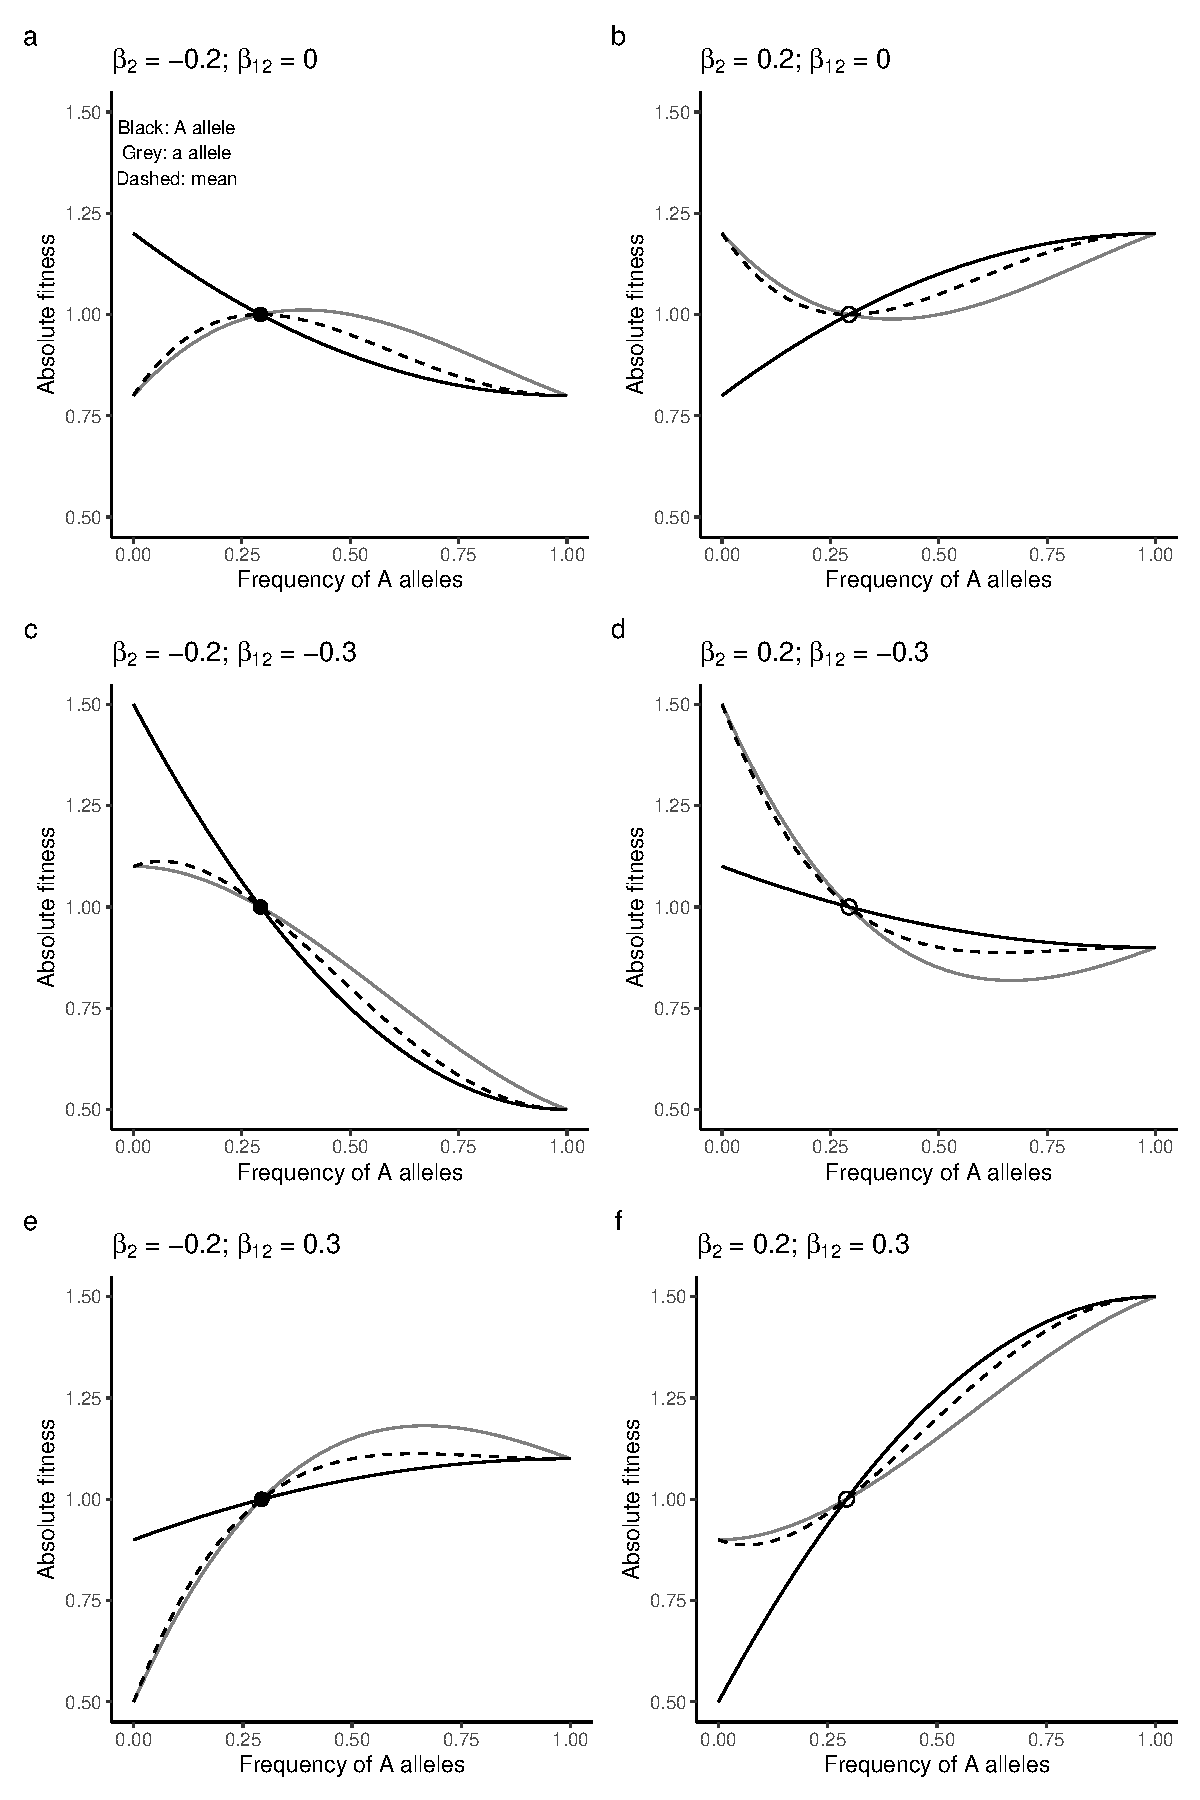
\includegraphics[width=0.7\linewidth]{AsymFDSdomi.pdf}
  \caption{Numerical examples for the fitness values $y_i$ in response to allele frequency when the A allele is completely dominant over the a allele. The black and gray lines indicate the marginal fitness of A and a alleles; that is, Equations (\ref{eq:5a}) and (\ref{eq:5b}), respectively. Dashed curves indicate the population-level mean fitness between the two alleles Equation (\ref{eq:6}). (a) Symmetric negative FDS; (b) Symmetric positive FDS; (c and e) asymmetric negative FDS; and (d and f) asymmetric positive FDS. Closed and open circles indicate a stable or unstable state, respectively. The base fitness and no directional selection were set at $\beta_0=1.0$ and $\beta_1=0.0$ for all panels.}
  \label{fig2:asym}
\end{figure}


While the Ising model poses an optimization problem of the total energy based on its interaction coefficient \citep{cipra1987introduction, anderson1991two, prugel1997dynamics}, evolutionary biologists have long analyzed optima of population-level mean fitness under FDS \citep{cockerham1972frequency,schneider_maximization_2008,takahashi2018balanced}. In a panmictic population, the population-level mean fitness is given by the allele-level marginal fitness weighted by its allele frequency (Appendix S3); that is, the weighted mean as follows.

\begin{equation}
\bar{y} = f y_\mathrm{A} + (1-f)y_\mathrm{a} = f^2 y_\mathrm{AA} + 2f (1-f)y_\mathrm{Aa} + (1-f)y_\mathrm{aa} \label{eq:6}
\end{equation}
\noindent
This population-level mean fitness is maximized at an intermediate frequency under symmetric negative FDS (Fig. \ref{fig2:asym}a) \citep{schneider_maximization_2008}. This expectation from randomly interacting and mating populations is comparable to the forward problem of the Ising model when $s_2<0$, where spatially mixed genotypes increase the population sum of $y_i$ more than monomorphic populations \citep{sato2019neighbor}. Even under an asymmetric negative FDS (Fig. \ref{fig2:asym}c and e), the population-level mean fitness became larger than expected by a weighted mean of monomorphic populations (= frequency-independent selection) \citep{takahashi2018balanced} (Fig. \ref{fig2:asym}c and e). In contrast, the population-level mean fitness was minimized at an intermediate frequency under a symmetric positive FDS (Fig. \ref{fig2:asym}b). Under asymmetric positive FDS, the population-level mean fitness was neither maximized nor greater than expected by frequency-independent selection \citep{schneider_maximization_2008, takahashi2018balanced} (Fig. \ref{fig2:asym}d and f). When A and a alleles showed additive expression as $x_{i(j)} \in$ \{AA, Aa, aa\} $=$ \{+1, 0, -1\}, fitness functions become so complicated that more than two equilibria might arise (Appendix S3; Figure \ref{figS2:FDSadd}) but have rarely been reported empirically. 


\subsection{Single-locus examples}
To test whether known FDS could be detected by our method, we applied the single-locus analysis Equations (\ref{eq:2}) and (\ref{eq:3}) to \textit{Arabidopsis} and \textit{Ischnura} data \citep{sato2017herbivore, takahashi2014evolution} collected under a split setting (Fig. \ref{fig1:scheme}a upper). The fitness components in the real data were in absolute values (e.g., number of eggs, flowers, and reproductive branches) where asymmetric FDS on the absolute fitness (Fig. \ref{fig2:asym}c-d) was possible in addition to symmetric FDS on relative fitness (Fig. \ref{fig2:asym}a and b). Therefore, symmetric and asymmetric FDS were tested using Equations (\ref{eq:2}) and (\ref{eq:3}), respectively. The lme4 package \citep{bates2015} in R was used for the single-locus analyses.

\subsubsection{Flower production of hairy and glabrous plants}
We applied single-locus analysis for the flower production data of \textit{Arabidopsis halleri} subsp. \textit{gemmifera} in order to detect known negative FDS mediated by leaf beetle attacks to hairy and glabrous plants \citep{sato2017herbivore}. The original data of \cite{sato2017herbivore} are downloaded from the Dryad repository (\url{https://doi.org/10.5061/dryad.53k2d}) and were re-analyzed using our proposed method. \cite{sato2017herbivore} set circular split plots (1 m in diameter) and recorded the trichome phenotype (hairy or glabrous), the number of flowers, leaf damage score, and the length of largest leaf for all individual plants within each plot. Field surveys were conducted along a 200-m line transect at the Omoide River, Hyogo, Japan (35$^\circ$06$^\prime$N, 134$^\circ$56$^\prime$E) from 2013 to 2016. The total sample size was 3,070 individuals among 324 plots. According to \cite{sato2017herbivore}, we used a generalized LMM (GLMM) with a Poisson error structure and a log-link function. The response variable was the number of flowers. The fixed effects were the self-phenotype (hairy or glabrous), similarity between the two morphs, and total number of plants within each field plot. The log-transformed length of the largest leaf (mm), which reflects the plant size, was included as an offset term. The random effects were the field plot IDs nested below the study years. In \textit{A. halleri}, hairy alleles are known to be dominant over glabrous alleles at the \textit{GLABRA1} locus \citep{shimizu2002ecology, kawagoe2011coexistence}. Given the complete dominance of hairy alleles over glabrous alleles, we assumed complete dominance at the \textit{GLABRA1} locus with $x_{i(j)} \in$ \{AA, Aa, aa\} $=$ \{+1, +1, -1\} on the basis of the trichome phenotype of an individual.

\subsubsection{Egg production of andromorph and gynomorph females in a damselfly}
We also applied single-locus analysis for the egg production of the blue-tailed damselfly \textit{Ischnura elegans} in order to detect known negative FDS and consequent increase in population-level mean fitness between an andromorph and a gynomorph \citep{takahashi2014evolution, le2015evolutionary}. The original data were derived from \cite{takahashi2014evolution} and consisted of 102 andromorphs and 79 \textit{infuscans}-type gynomorphs. \cite{takahashi2014evolution} assigned adult \textit{I. elegans} with an andromorph frequency of 0.2, 0.5, or 0.8 into split-field cages under low- or high-density conditions. This field experiment was conducted at the Stensoffa Field Station of Lund University. According to \cite{takahashi2014evolution}, we used a GLMM with a Poisson error structure and a log-link function. The response variable was the number of mature eggs. The fixed effects were morph type and morph similarity within a cage. The cage ID and experimental ID were considered random effects, where the cage ID was nested below the experimental ID. The andromorph allele is known to be dominant over the \textit{infuscans}-type gynomorph allele on an autosomal locus \citep{sanchez2005hybridization}. Therefore, on the basis of phenotype frequencies within the split cages, we assumed complete dominance with genotype values encoded as $x_{i(j)} \in$ \{AA, Aa, aa\} $=$ \{+1, +1, -1\} for homozygous andromorphs, heterozygous andromorphs, and homozygous gynomorphs, respectively. The interaction term between the morph type and similarity was also considered in the line of GLMMs to test the significance of asymmetric FDS between the two morphs. If the interaction term was not significant, the coefficients of the main effect were estimated using GLMM without any interaction terms.


\subsection{GWAS simulation}
Simulations were performed to evaluate the power of our method for detecting causal polymorphisms from genome-wide SNPs. The entire procedure consisted of three steps: We (i) simulated genomic structure under balancing selection, (ii) conducted virtual experiments to simulate fitness from the simulated genomes, and (iii) applied our method for GWAS of simulated fitness and genomes. We used Equation (\ref{eq:2}) to focus on symmetric FDS on relative fitness in this simulation because selection acted not on absolute but on relative fitness. To test the notion that linear mixed models (LMMs) usually outperform standard linear models (LMs) in GWAS \citep{kang2008efficient}, we compared the performance of LMs [Equation (\ref{eq:2})] to LMMs (see Appendix S2 for the mixed model extension). We used SLiM version 3 \citep{haller_slim_2019} for population genetic simulations; and the vcfR \citep{knaus2017vcfr}, gaston \citep{R_gaston}, rNeighborGWAS \citep{sato2019neighbor}, and pROC \citep{R_pROC} packages in R version 4.0.3 \citep{R_citation} for GWAS mapping.

\subsubsection{Simulated genomes}
Population genetic simulations were performed using the SLiM version 3 to create a realistic genome structure. Running 30 independent iterations for 2000 generations, we simulated 50 kb nucleotide $\times$ three chromosomes $\times$ 10 subpopulations $\times$ 200 individuals. Base parameters were set at the mutation rate $\mu = 10^{-6}$, selection coefficient $s_1=s_2=0.1$ for non-neutral mutations, and recombination rate $r=10^{-5}$. Ten subpopulations were distributed in a circle with a low migration rate $m=10^{-4}$ between neighboring populations. In this simulation, we decomposed the total fitness as $w_i = w_{i,1} + w_{i,2}$. The first fitness component $w_{i,1}$ involves self-genotype effects $\beta_1$, and $w_{i,2}$ is the second fitness component subject to the power analysis of genotype similarity effects $\beta_2$. For the self-genotype effects $\beta_1$, we define stabilizing selection as $w_{i,1} = 1.5 - [(z_{i,1} - z_1^*)^2 / s_1N_k]$, where $z_1^*$ is the optimum number of QTLs responsible for self-genotype effects per genome per population, and $z_i$ is the number of QTLs for individual $i$. We set $z_1^*$ to five and assumed additive effects by the QTLs. Following the standard way to simulate polygenic selection \citep{haller_slim_2019}, we did not allow the substitution of QTLs for $w_{1,i}$ even after they were fixed. For the genotype similarity effects $\beta_2$, we assumed four specific scenarios of selection on the second fitness component $w_{i,2}$ as follows: 

Scenario 1. Negative frequency-dependent selection: For the test of $\beta_2$, we simulated negative FDS on the second fitness component $w_{i,2}$. We simulated negative FDS for the second fitness component as $w_{i,2} = 1.5 - s_ 2 g _if_k$, where $f_k$ indicates the frequency of the mutation within a subpopulation $k$. Novel mutations were assumed to be recessive to ancestral alleles with genotype $g_i$ redefined as $g_i \in$ \{AA, Aa, aa\} $=$ \{1, 1, 0\}. Polymorphisms were likely balanced under negative FDS; thus, the mutation rate was set at half of the base parameter to maintain the number of causal SNPs in the same order as in the other scenario.

Scenario 2. Positive frequency-dependent selection: We also simulated the opposite regime, positive FDS, on the second fitness component $w_{i,2}$. It is known that locally acting positive FDS within a subpopulation can lead to global coexistence of two alleles among subpopulations \citep{molofsky2001coexistence}. Therefore, we separated the entire population into four panmictic subpopulations to simulate polymorphic loci. Similar to the negative FDS, we simulated positive FDS as $w_{i,2} = 1.5 + s_ 2 g _if_k$. Novel mutations were assumed to be recessive to ancestral alleles with genotype $g_i$ redefined as $g_i \in$ \{AA, Aa, aa\} $=$ \{1, 1, 0\}. 

Scenario 3. Overdominance: To test whether $\beta_2$ confounded frequency-independent types of balancing selection, we simulated genomes under overdominance selection. The second fitness component is defined as $w_{i,2} = 1.5 + s_2hg_i$, where $h$ is the dominance coefficient expressed on the basis of genotypes as \{$h_\mathrm{AA}, h_\mathrm{Aa}, h_\mathrm{aa}$\} $=$ \{1.0, 2.0, 1.0\}.

Scenario 4. Spatiotemporally varying selection: To test another type of frequency-independent balancing selection, we simulated genomes under spatiotemporally varying selection. The second fitness component is defined as $w_{i,2} = 1.5 + s g_i$, where $s$ varies in space and time. We assumed $s_2=0.1$ for two subpopulations, and $s_2=-0.1$ for the other two subpopulations. For six of the four subpopulations, we changed the selection coefficient in time to $s_2=0.1$ for odd generations and $s_2=-0.1$ for even generations. We reset $m=0.001$ to allow a higher migration rate. In this scenario, novel mutations were assumed to be recessive to ancestral alleles.

\subsubsection{Virtual experiments}
We then sampled the simulated genomes and generated fitness values from the genotype data. The simulated genomes were exported in variant call format (.vcf) and loaded into R using the vcfR package \citep{knaus2017vcfr}. SNPs were filtered with a cut-off threshold of minor allele frequency (MAF) of 0.01. We assumed two experimental settings: split and continuous populations (Fig. \ref{fig1:scheme}a). To describe the two distinct cases, 900 individuals were randomly sampled from each simulation without replacement and assigned to a 30 $\times$ 30 lattice space for the continuous setting, or 10 individuals each to 90 split cages for the split setting.

Fitness values were then simulated from the simulated genomes and their spatial arrangement. To calculate the self-genotype component $\beta_1x_i$ in Equation (\ref{eq:2}), we assigned 0.1 (which corresponded to the selection coefficient $s_1$ in the population genetic simulation) to $\beta_1$ of causal SNPs or zero to those of the other SNPs. The second fitness component at causal SNPs was generated with $\beta_2 = 0.1$ (corresponding to the strength of balancing selection $s_2$ in the population genetic simulation), for negative or positive FDS as $(\pm \beta_2\sum^{N_{k}}_{j=1}{x_ix_j}) / 2N_k$; for overdominance as $x_i \in$ \{AA, Aa, aa\} = \{$1+\beta_2, 1+\beta_2h, 1$\}, and for spatiotemporally varying selection as a random assignment of $\pm \beta_2$ to $\beta_2x_i$. Fitness variance was not adjusted for the first and second fitness components, since the number of causal SNPs and their effect sizes were controlled during the population genetic simulation above. Gaussian residual errors were finally added to the simulated fitness such that approximately one-third of the total phenotypic variation was attributed to the environmental variance as Var($\mathbf{e}$) $=(0.75)^2 \times$Var($\mathbf{w}$). This range of the number of causal SNPs and the proportion of phenotypic variation explained by the model was based on parameter settings where the model performance was well differentiated \citep{sato2019neighbor}.

\subsubsection{GWAS using simulated genomes and fitness}
Finally, we performed association mapping of the simulated fitness with respect to $\beta_1$ and $\beta_2$. The rNeighborGWAS package \citep{sato2019neighbor} was used to implement the regression model in Equation (\ref{eq:2}) as an LMM (Appendix S2). The false vs. true positive rate was analyzed using the receiver operating characteristic (ROC) curve. Similar to the generative model, we assumed the dominant encoding for the three genotypes, $x_{i(j)} \in$ \{AA, Aa, aa\} $=$ \{+1, +1, -1\}. To measure the efficiency of causal polymorphism detection, we calculated the area under the ROC curve (AUC) for the -log\textsubscript{10}($p$-values) of $\beta_1$ or $\beta_2$. The AUC ranged from 0.5 (no power to detect causal SNPs) to 1.0 (perfect matching between the top $p$-value score and causal SNPs). To measure the accuracy of the effect size estimates, we compared the true and estimated values of $\beta_2$. To test if LMMs could outperform standard (LMs), we also compared AUCs and $\hat{\beta}_2$ between LMM and LM.


\subsection{Pilot GWAS}
To examine whether our method is applicable to real GWAS dataset, we conducted a pilot GWAS of reproductive branch number in  field-grown \textit{A. thaliana} under a continuous setting (Fig. \ref{fig1:scheme}a lower). According to \cite{sato2019plant}, a summer cohort composed of natural accessions with various life cycles was established to investigate the survival and reproduction under stressful environments. We selected 199 worldwide accessions from 2029 inbred lines sequenced by the RegMap \citep{horton_genome-wide_2012} and 1001 Genomes project \citep{alonso-blanco_1135_2016}. Full-imputed genotypes were downloaded from the AraGWAS catalog \citep{togninalli_aragwas_2018}. For the 199 accessions, 1,819,577 SNPs were selected at a cut-off threshold of MAF $>$ 0.05. Three replicates of the 199 accessions were sown on Jiffy-seven (33 mm in diameter) and stratified under constant dark conditions with a 4C$^{\circ}$ air temperature for a week. Seedlings were first grown under short-day conditions (8 L: 16D, 20C$^{\circ}$) for 6 weeks. Individual plants were then potted into a plastic pot (6 cm in diameter) filled with mixed soils of agricultural compost (Profi Substrat Classic CL ED73, Einheitserde Co.) and perlite with a 3:1 L ratio of perlite. Potted plants were transferred to the common garden at the Irchel Campus of the University of Zurich (Zurich, Switzerland: 47$^\circ$23$^\prime$N, 08$^\circ$33$^\prime$E) on 8 July 2019. In the field setting, a set of 199 accessions and an additional Col-0 accession were randomly assigned to each block without replacement. The 200 plants were set in plastic trays (10 $\times$ 40 cells in a continuous space) in a checkered pattern. Three replicates of each block were set $>$ 1.5 m apart from each other. We recorded the length of the largest leaf (mm) at the start of the experiment, the presence of bolting after 2 weeks, and the branch number at the end of the experiment (27 August 2019). We considered the branch number as a proxy for fitness, because it is known as a major fitness component of \textit{A. thaliana} \citep{chong2018note}, and other reproductive phenotypes were difficult to observe owing to the stressful summer environment. Dead plants were recorded as a branch number of zero \textit{ that is }, with no fitness. Accession names and phenotype data are presented in Table \ref{tableS3:GWASdata}.

The branch number was analyzed as a target trait of GWAS. The rNeighborGWAS package version 1.2.3 \citep{sato2019neighbor} was used to implement Equations (\ref{eq:2}) and (\ref{eq:3}) as GWAS (Appendix S2). The inbred lines of \textit{A. thaliana} have either AA or aa genotype, in which the qualitative interpretation of $\beta_2$ and $\beta_{12}$ in this inbred case remains the same as in the case of complete dominance (Appendix S3; Figure \ref{figS3:FDSinbred}). The response was log(x+1)-transformed number of branches. We assumed that FDS arose from genetic interactions among neighboring plants in small \textit{Arabidopsis}, and thus the genotype similarity was considered up to the nearest neighbors; that is, $N_k=4$ from a focal individual. The initial plant size, presence of bolting, experimental block ID, and edge of each plot (or not) were considered as non-genetic covariates. The marker kinship and genome-wide structure of neighbor genotype similarity were considered random effects. After association mapping, we focused on SNPs with a -log\textsubscript{10}(\textit{p}-value) score $>$ 4.0. We searched candidate genes within $\sim$10 kb around the target SNPs, based on the Araport11 gene model with the annotation of The Arabidopsis Information Resource (TAIR; accessed on 31 December 2021). Gene ontology (GO) enrichment analysis was performed using the Gowinda algorithm \citep{kofler2012gowinda} with the options “--gene-definition undownstream1000,” “--min-genes 2,” and “--mode gene.” The GO.db package \citep{Carlson2020GOdb} and the latest TAIR AGI code annotations were used to build the input files.


\section{Results}

\subsection{Negative FDS on trichome dimorphism in \textit{A. halleri}}
To test whether the single-locus analysis could detect known negative FDS, we applied Poisson GLMM for the flower production data on hairy and glabrous plants of \textit{A. halleri} under the split setting of field plots \citep{sato2017herbivore}. The Poisson GLMM detected a negative and significant coefficient of the morph similarity $\hat{\beta}_2$ (Table \ref{table1:GLMM}a), indicating negative FDS where a focal plant produced more flowers as dissimilar morphs were grown within the same plot. The lack of significance of the interaction term between the trichomes and morph similarity suggest that negative FDS is symmetric between hairy and glabrous plants (Table \ref{table1:GLMM}a). We also found the same level of the self-morph coefficient $\hat{\beta}_1$ as the negative coefficient of morph similarity $\hat{\beta}_2$ (Table \ref{table1:GLMM}a), indicating the simultaneous action of directional selection and negative FDS between the two morphs. However, the total number of plants, namely the density, had no significant effect on flower production (Table \ref{table1:GLMM}a). The fitness function estimated from $\hat{\beta_0}, \hat{\beta_1}, \hat{\beta_2}$, and $\hat{\beta}_{12}$ showed that a stable equilibrium under negative FDS remained at a biased but not monomorphic frequency (Fig. \ref{fig3:GLMM}a). This discrepancy between the observed frequency and expected equilibrium was likely because the present selection analysis could not incorporate another major component of fitness in \textit{A. halleri} \textit{that is} clonal reproduction \citep{sato2017herbivore}. These results provide qualitative evidence for negative FDS on trichome dimorphism through the fitness component of flower production.

\begin{figure}[ht]
  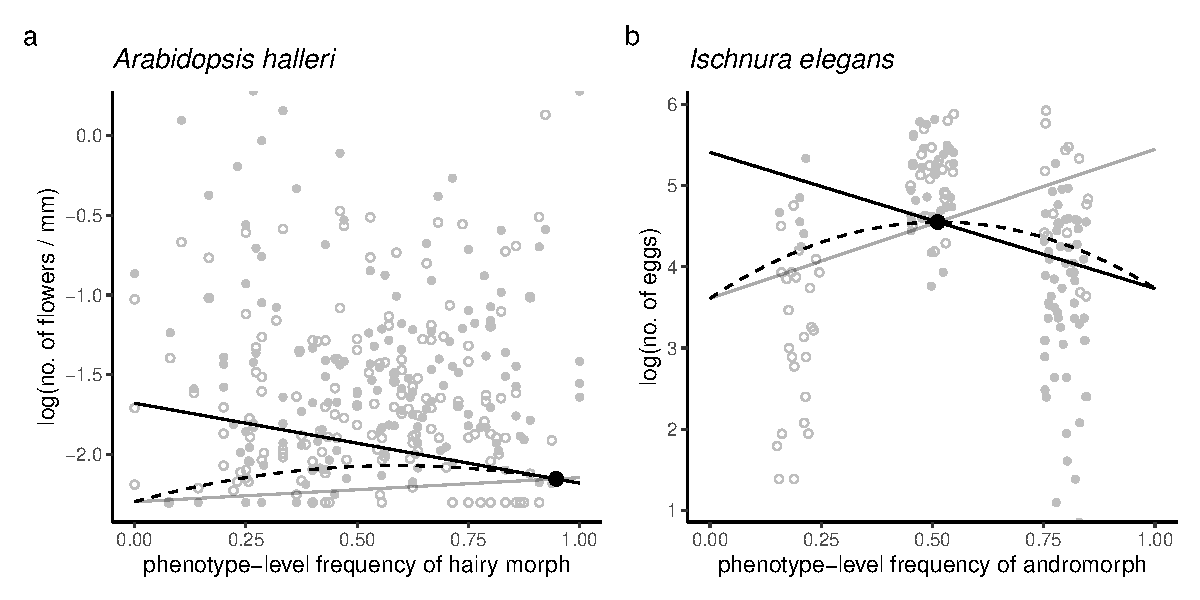
\includegraphics[width=0.75\linewidth]{Ah_Ie_plots.pdf}
  \caption{Negative frequency dependence in (a) the size-adjusted number of flowers in \textit{A. halleri} and (b) the number of mature eggs in \textit{I. elegans}. Fitness functions are based on the estimates from Table \ref{table1:GLMM} and are shown at a phenotype level (see case 3 in Appendix S3) to project model trends on the observed fitness. Black and white lines indicate the fitness function of dominant (i.e., hairy and andromorph) or recessive (glabrous and gynomorph) morphs, respectively. Filled and open circles indicate the observed fitness for the dominant or recessive morph within a plot, respectively. The dashed curve shows population-level mean fitness. The black dot represents a stable equilibrium under negative FDS. In panel (a), a single circle corresponds to a field plot, where the average number of flowers adjusted by plant size (mm) among hairy or glabrous plants is given after log($x$+0.1)-transformed.}
  \label{fig3:GLMM}
\end{figure}

\begin{table}[ht]
\caption{Poisson generalized linear mixed model (GLMM) applied to the number of flowers between hairy and glabrous \textit{A. halleri} (a) or the number of mature eggs between the andromorph and gynomorph of \textit{I. elegans} (b). Morph similarity was calculated from the genotype similarity defined by Equation (\ref{eq:2}). Estimated coefficients, their standard errors (SE), $Z$-values, and $p$-values are shown for multiple regressions. Bold letters indicate significance at $p<$ 0.05 by Wald tests.}
(a) \textit{Arabidopsis halleri} \\
\begin{tabular}{lllll}
\hline
\multicolumn{1}{c}{Fixed effects} & \multicolumn{1}{c}{Coefficient} & \multicolumn{1}{c}{SE} & \multicolumn{1}{c}{\textit{Z}} & \multicolumn{1}{c}{\textit{p}} \\ \hline
\textbf{Intercept} $\hat{\beta}_{0}$    & \textbf{-2.076}  &  \textbf{0.17} & \textbf{-11.97} & \textbf{\textless{}2e-16}  \\
\textbf{Self-morph} $\hat{\beta}_{1}$      & \textbf{0.146}                  & \textbf{0.008}         & \textbf{17.32}                 & \textbf{\textless{}2e-16}      \\
\textbf{Morph similarity} $\hat{\beta}_{2}$        & \textbf{-0.163}                 & \textbf{0.018}         & \textbf{-9.22}                 & \textbf{\textless{}2e-16}      \\
Total no. of plants               & -0.006                          & 0.010                  & -0.63                          & 0.53                           \\
Self $\times$ Similarity $\hat{\beta}_{12}$            & -0.088                          & 0.048                  & -1.81                          & 0.07                           \\ \hline
\end{tabular}

\vspace*{5mm}

(b) \textit{Ischnura elegans} \\
\begin{tabular}{lllll}
\hline
\multicolumn{1}{c}{Fixed effects} & \multicolumn{1}{c}{Coefficient} & \multicolumn{1}{c}{SE} & \multicolumn{1}{c}{\textit{Z}} & \multicolumn{1}{c}{\textit{p}} \\ \hline
\textbf{Intercept} $\hat{\beta}_{0}$    & \textbf{4.55} &  \textbf{0.191} & \textbf{23.8}  & \textbf{\textless{}2e-16}  \\
\textbf{Self-morph} $\hat{\beta}_{1}$               & \textbf{-0.021}                 & \textbf{0.008}         & \textbf{-2.56}                 & \textbf{0.01}                  \\
\textbf{Morph similarity} $\hat{\beta}_{2}$           & \textbf{-0.878}                 & \textbf{0.022}         & \textbf{-39.30}                & \textbf{\textless{}2e-16}      \\
Density                             & 0.097                           & 0.237                  & 0.41                           & 0.68                           \\
Self $\times$ Similarity $\hat{\beta}_{12}$                 & -0.042                          & 0.25                 & -0.17                          & 0.87                           \\ \hline
\end{tabular}
\label{table1:GLMM}
\end{table}

\subsection{Negative FDS on female color polymorphisms in \textit{I. elegans}}
To further test whether the single-locus analysis could represent a known relationship between negative FDS and population-level mean fitness, we applied Poisson GLMM for the data on the number of mature eggs between the andromorph and gynomorph of \textit{I. elegans} under the split setting of field cages \citep{takahashi2014evolution}. Consistent with the previous evidence for negative FDS \citep{van2001frequency, le2015evolutionary}, we found a significantly negative coefficient of morph similarity $\hat{\beta}_2$ (Table \ref{table1:GLMM}b). The interaction term between the morph type and similarity was not significant (Table \ref{table1:GLMM}b), indicating no significant asymmetry in the negative FDS between the two morphs. We also found a significant effect of morph type (andromorph or gynomorph) on the egg number, but its effect was much less significant than that of morph similarity (Table \ref{table1:GLMM}b). As reported in a previous study \citep{takahashi2014evolution}, the density did not significantly affect the egg number (Table \ref{table1:GLMM}b). The fitness function estimated from $\hat{\beta_0}, \hat{\beta_1}, \hat{\beta_2}$, and $\hat{\beta}_{12}$ shows that negative FDS allows the two morphs to coexist at an intermediate frequency (Fig. \ref{fig3:GLMM}b). Consistent with the results of \cite{takahashi2014evolution}, the population-level mean fitness increased at a stable equilibrium at the intermediate frequency (Fig. \ref{fig3:GLMM}b). These results support the action of symmetric negative FDS and the consequent increase in the population-level mean fitness. Taken together, \textit{A. halleri} and \textit{I. elegans} data suggest that our single-locus model can be applied to selection gradient analyses of FDS on visible polymorphic traits that follow typical Mendelian inheritance with complete dominance (see also the discussion "Selection gradient along genotype similarity").

\begin{figure}[ht]
  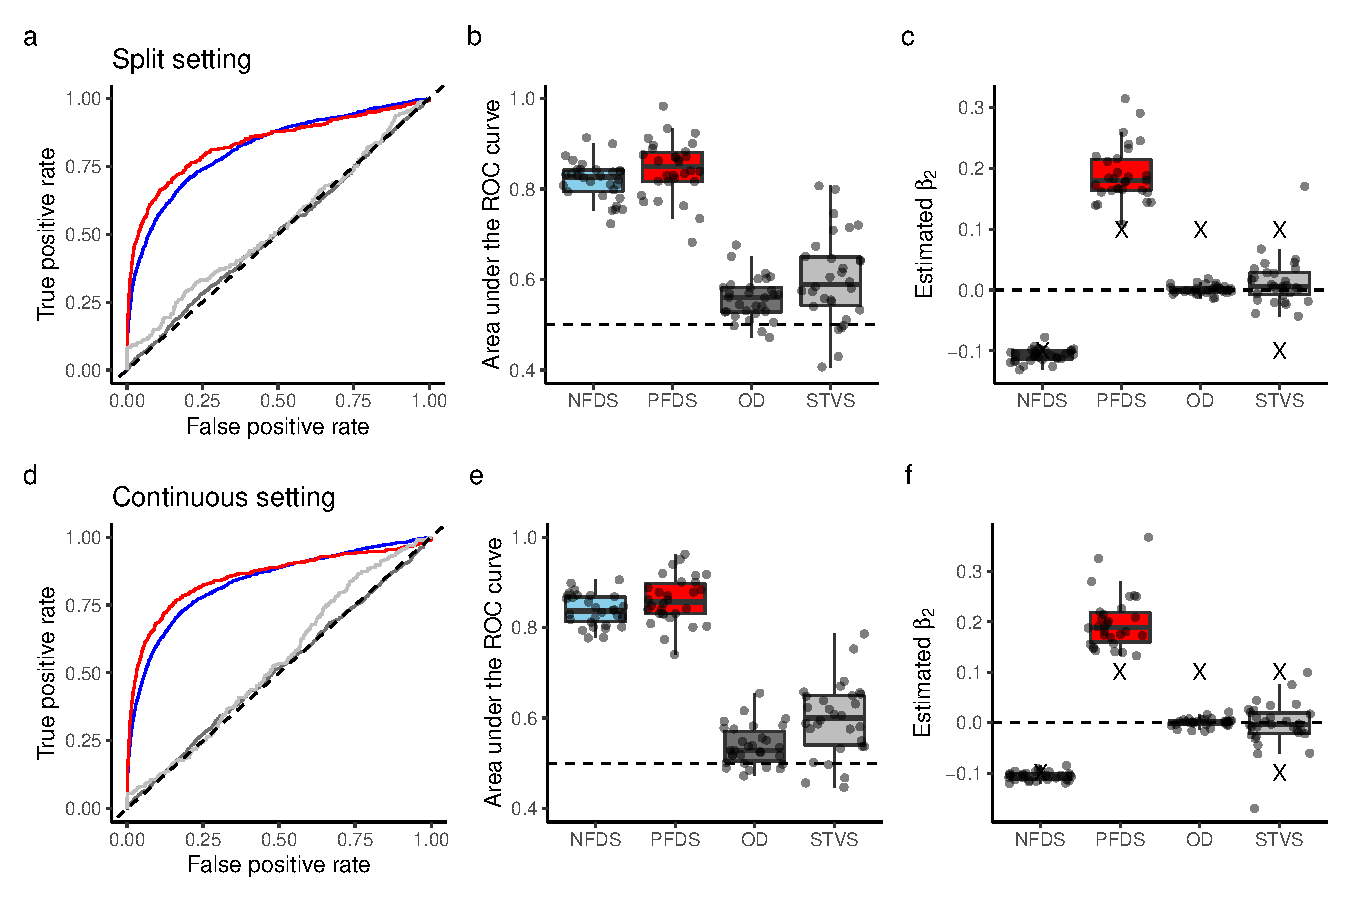
\includegraphics[width=0.7\linewidth]{beta2LMMdomi.pdf}
  \caption{Performance of linear mixed models to estimate four types of simulated selection: NFDS, negative frequency-dependent selection (blue); PFDS, positive frequency-dependent selection (red); OD, overdominance (dark gray); and STVS, spatiotemporally varying selection (light gray). The upper and lower panels show the results of the split and continuous settings, respectively (Fig. \ref{fig1:scheme}a). The left panels (a) and (b) show the receiver operating characteristic (ROC) curve, which indicates the relationship between the true positive rate and false positive rate. The middle panels (b) and (e) shows the area under the ROC curve (AUC). Dashed lines at AUC = 0.5, indicate no power to detect causal single nucleotide polymorphisms (SNPs). The right panels (c) and (f) show the estimated $\beta_2$ of causal SNPs, where negative and positive values indicate negative and positive FDS, respectively. Cross marks indicate the true simulated magnitude of $\beta_2$. Boxplots show the median by a center line, upper and lower quartiles by box limits, and 1.5$\times$ interquartile range by whiskers.}
  \label{fig4:beta2LMM}
\end{figure}

\subsection{Detection of simulated FDS across a genome}
We simulated genotypes and fitness to test whether our method could distinguish negative FDS, positive FDS, overdominance, and spatiotemporally varying selection among genome-wide SNPs. The simulated genomes had 2,000 to 4,500 SNPs with MAFs $>$ 0.01 across 50 kbp nucleotide sequences (Fig. \ref{figS4:GenStr}). They exhibited low heterozygosity (\textit{H}\textsubscript{t} $<$ 0.1) and moderate to strong differentiation among 10 populations (\textit{G}\textsubscript{st} $<$ 0.5; Fig. \ref{figS4:GenStr}c), where approximately 200 SNPs were involved in polygenic stabilizing selection (Fig. \ref{figS4:GenStr}a). Regarding the causal SNPs, SNPs responsible for positive FDS showed strong population structures (\textit{G}\textsubscript{st} $>$ 0.8) with low heterozygosity (\textit{H}\textsubscript{t} $<$ 0.05; Fig. \ref{figS4:GenStr}b) because positive FDS disrupts polymorphisms within a population. In contrast, because negative FDS maintains polymorphisms within a population, SNPs responsible for negative FDS had weak population structures (\textit{G}\textsubscript{st} $<$ 0.2) with high heterozygosity (\textit{H}\textsubscript{t} $>$ 0.35; Fig. \ref{figS4:GenStr}b).

We implemented the single-locus model Equation (\ref{eq:2}) as a linear mixed model (LMM) for GWAS (Appendix S2), and evaluated the performance of LMMs in terms of causal polymorphism detection and effect size estimates (Fig. \ref{fig4:beta2LMM}). The power to detect negative and positive FDS was strong (median AUC $>$ 0.8) in both the split and continuous settings (Fig. \ref{fig4:beta2LMM}a, b, d and e). The direction of the FDS matches the estimated sign of $\beta_2$ (Fig. \ref{fig4:beta2LMM}c and f). In contrast, our method had almost no power to detect overdominance (Fig. \ref{fig4:beta2LMM}b and e). Compared with overdominance, spatiotemporally varying selection was more likely, but the power remained weak (median AUC $<$ 0.6) and its estimated coefficients had a median value of almost zero (Fig. \ref{fig4:beta2LMM}b-c and e-f). These results indicate that our method retains the power to detect negative and positive FDS in GWAS, with other types of balancing selection less likely confounded. 

The performance of LMMs was compared with that of standard LMs (Fig. \ref{fig4:beta2LMM}, Fig. \ref{figS5:beta2LM}). In terms of AUC, LMMs outperformed LMs in the detection of negative FDS (Fig. \ref{fig4:beta2LMM}b and e, Fig. \ref{figS5:beta2LM}b and e). Although LMs and LMMs exhibited similar performances for positive FDS, LMs overestimated the true strength of positive FDS more than LMMs (Fig. \ref{fig4:beta2LMM}c and f, Fig. \ref{figS5:beta2LM}c and f). LMMs retained a slight power to detect polygenic stabilizing selection (weakly concave ROC curve; Fig. \ref{figS6:beta1LMM}a and d), whereas LMs had almost no power to detect the stabilizing selection (almost flat ROC curve; Fig. \ref{figS7:beta1LM}a and d). These results suggest that LMMs suit the proposed method because they can more efficiently capture negative FDS or prevent overestimation of the strength of positive FDS.

\subsection{Field GWAS of the branch number in \textit{A. thaliana}}
To examine the feasibility using real GWAS dataset, we finally applied an LMM for field GWAS of the branch number in \textit{A. thaliana} (Fig. \ref{fig5:gwas}) under the continuous setting (Fig. \ref{fig1:scheme}a lower). QQ-plots exhibited little inflation of the observed $p$-value score against the expected score (Fig. \ref{figS9:QQplotLMM}). Of 561 plants, 181 bolted 2 weeks after they were transferred to the field in July. The proportion of branch number variation explained by self-genotypes $(=\hat{\sigma}^2_1/(\hat{\sigma}^2_1 + \hat{\sigma}^2_e))$ was 0.68, indicating high heritability of the fitness component. For the self-genotype effects $\beta_1$ (i.e., standard GWAS), we detected no significant SNPs above the Bonferroni threshold but found a peak on the top of chromosome 4 (Fig. \ref{fig5:gwas}a; Table \ref{tableS4:GWAScandidates}a). The top of chromosome 4 is known to encompass a flowering QTL and natural variation in the \textit{FRI} \citep{aranzana2005genome}. GO enrichment analysis detected no significant annotations at a false discovery rate of $<$ 0.05. 

\begin{figure}[ht]
  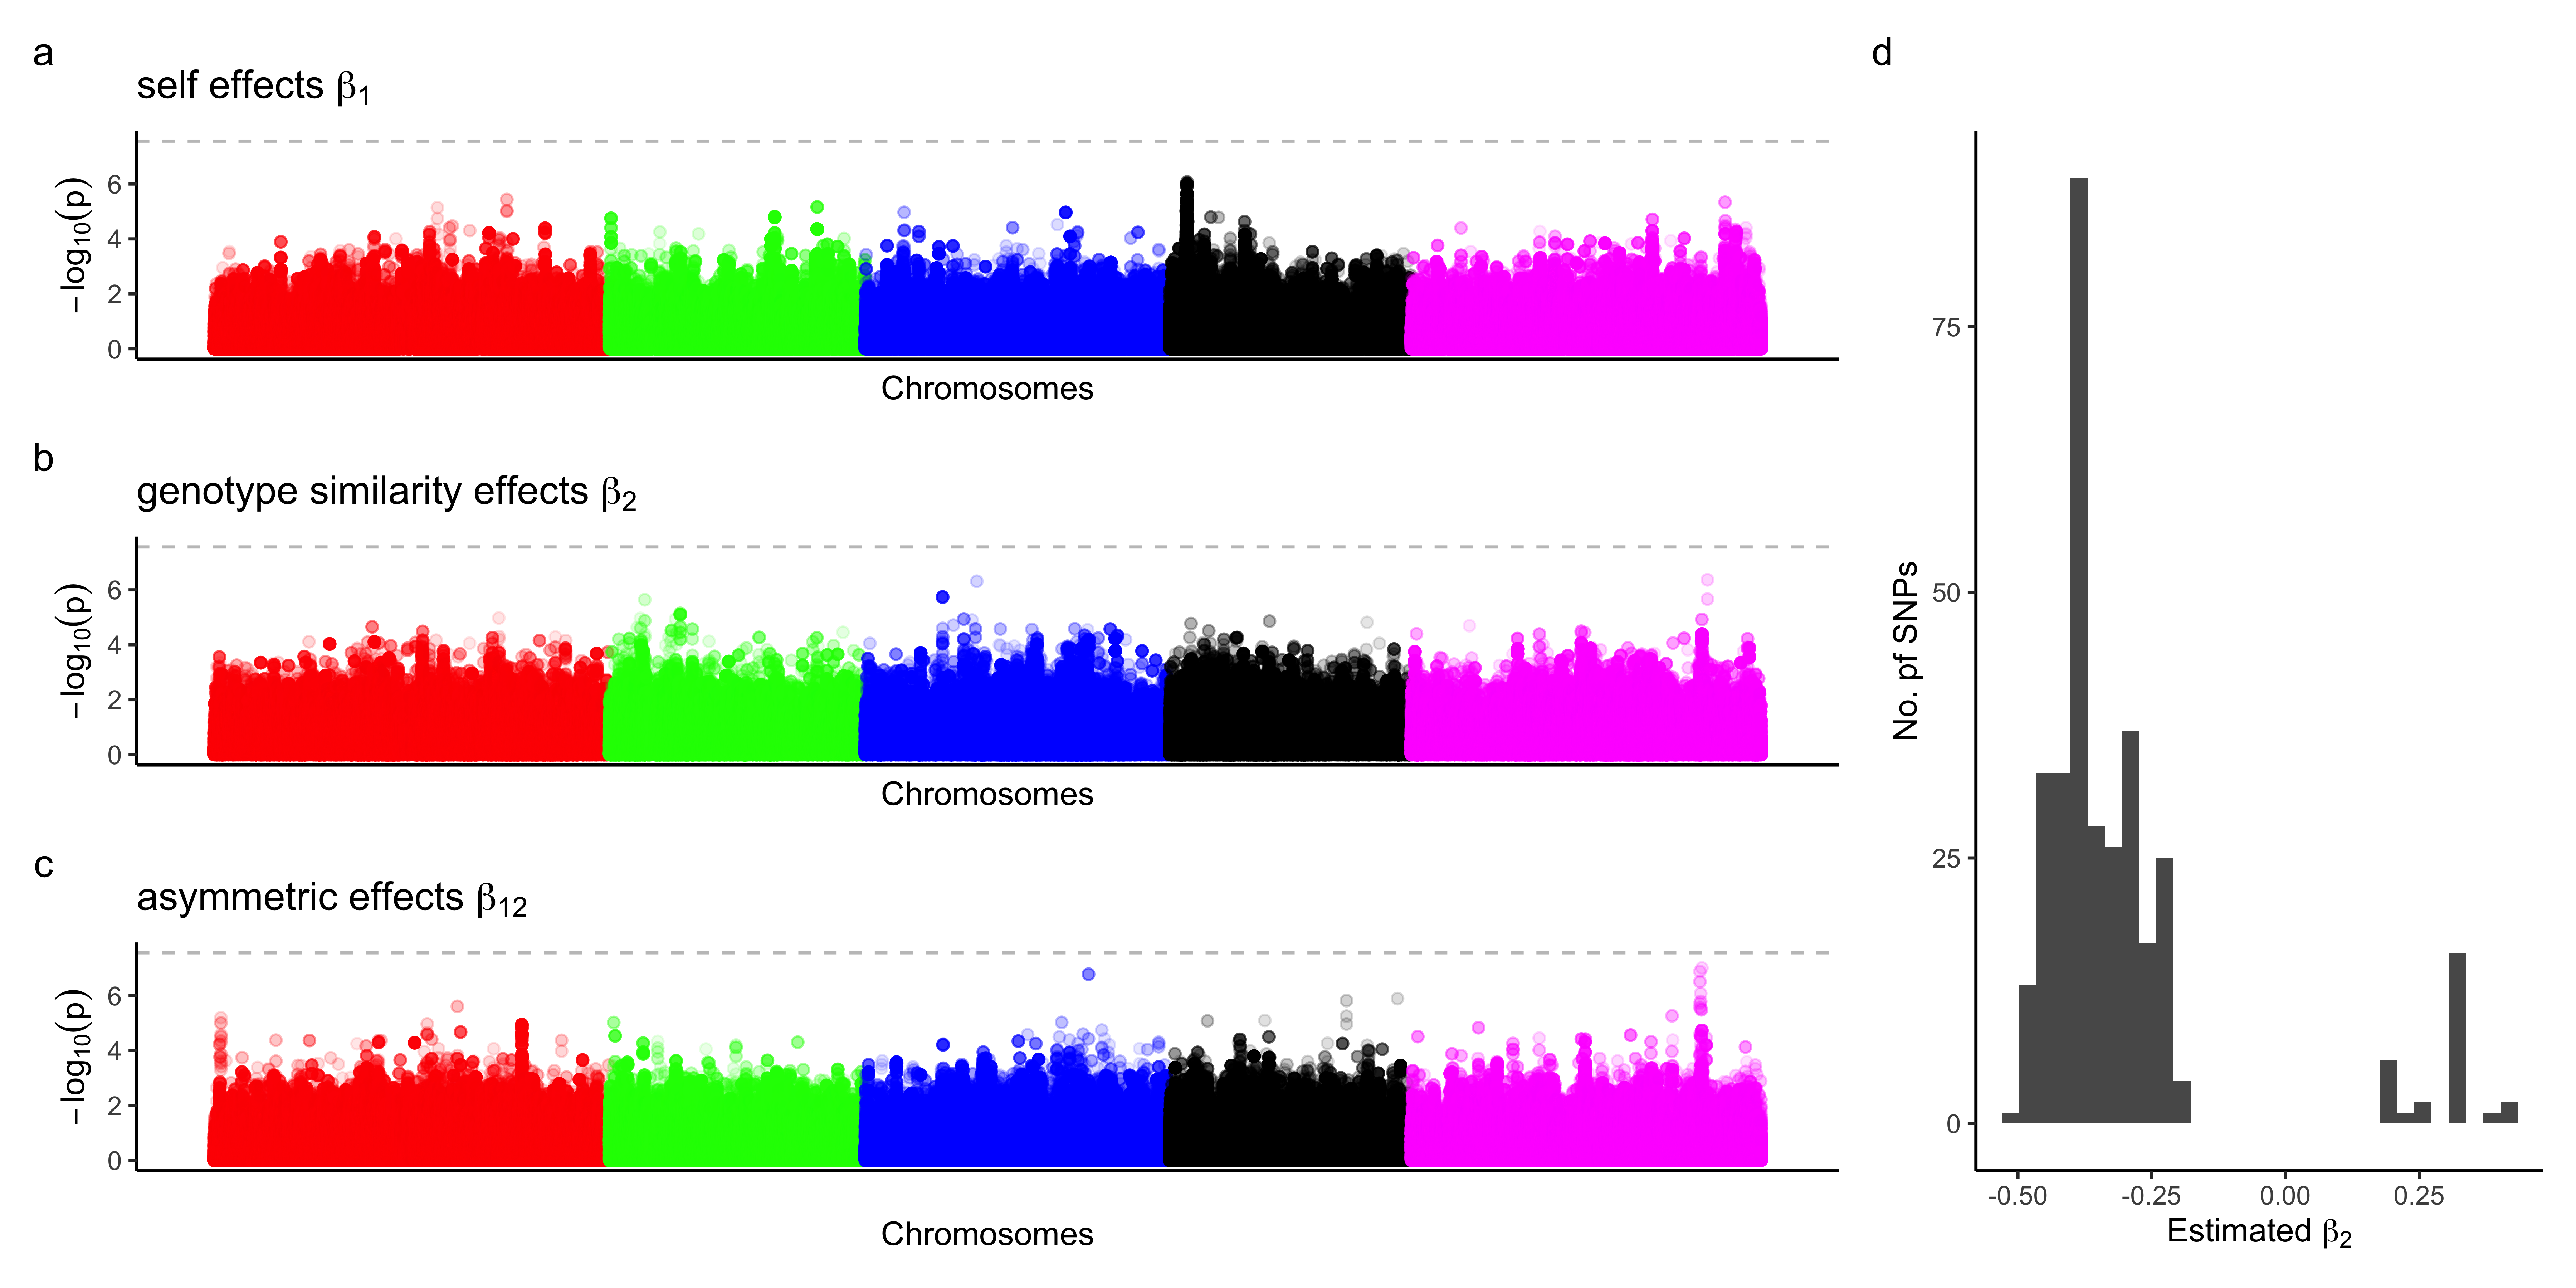
\includegraphics[width=\linewidth]{ManhattanLMM.png}
  \caption{Genome-wide association studies of branch number in field-grown \textit{Arabidopsis thaliana} under the continuous population setting (Fig. \ref{fig1:scheme}a lower). The results of linear mixed models are shown. (a, b, and c) Manhattan plots for self-genotype effects, genotype similarity effects, and asymmetric effects, respectively. Horizontal dashed lines indicate $p$-value $=$ 0.05, after Bonferroni correction. (d) Histogram of estimated $\beta_2$ among SNPs exhibiting $p$-values $<$ 0.0001. Negative and positive $\beta_2$ infer loci responsible for negative and positive FDS, respectively.}
  \label{fig5:gwas}
\end{figure}

For the genotype similarity effects $\beta_2$, we also found no significant SNPs but top-scoring SNPs on chromosomes 3 and 5 (Fig. \ref{fig5:gwas}b). Within 10 kbp near the top-scoring SNP on chromosome 3, we observed the \textit{GAE6} gene, which encodes a UDP-D-glucuronate 4-epimerase involved in pectin biosynthesis, cell wall integrity, and immunity to pathogens \citep{bethke2016pectin}. To elucidate genome-wide patterns of $\beta_2$ and candidate genes, we focused on SNPs exhibiting $p$-values of $<$ $10^{-4}$, corresponding to smaller than 0.025 percentiles. Of the 254 SNPs selected, 195 and 59 showed negative and positive $\beta_2$, respectively (Fig. \ref{fig5:gwas}d). Genes involved in plant immunity and resistance, such as \textit{GAE6}, \textit{ARGONAUTE 4} (\textit{AGO4}), and \textit{ACTIVATED DISEASE RESISTANCE 1} (\textit{ADR1}), were observed within 10 kb near the SNPs showing negative $\beta_2$ at $p$-value $<$ 0.0001 (Table \ref{tableS4:GWAScandidates}b). In contrast, \textit{AVRRPT2-INDUCED GENE 1} (\textit{AIG1}) was only a resistance-related gene observed near the SNPs showing positive $\hat{\beta}_2$ at $p$-values of $<$ 0.0001 (Table \ref{tableS4:GWAScandidates}b). GO enrichment analysis found no significant GO annotations at a false discovery rate of $<$ 0.05.

We also tested the asymmetric effects $\beta_{12}$ for all SNPs by detecting a QTL on chromosome 5 near the Bonferroni threshold (Fig. \ref{fig5:gwas}c). These SNPs exhibited positive $\beta_2$ and $\beta_{12}$ (i.e., $\hat{\beta}_2=0.78$ and $\hat{\beta}_{12}=1.13$ on chromosome 5 at position 22382673: Table \ref{tableS4:GWAScandidates}c), indicating positive effects of a reference allele on absolute fitness together with positive FDS on relative fitness. Genes potentially related to growth were located near this top-scoring SNP, including \textit{SUMO2} and \textit{SUMO3}. GO enrichment analysis found no significant GO annotations at a false discovery rate of $<$ 0.05.

To compare the LMMs and LMs, we applied standard linear models for the branch number (Fig. \ref{figS10:gwasLM}). For the self-genotype effects, a large number of SNPs showed larger -log\textsubscript{10}($p$-values) scores than the Bonferroni threshold (Fig. \ref{figS10:gwasLM}a). The observed $p$-values for the self-genotype effects were greater than expected (Fig. \ref{figS11:QQplotLM}a), showing that LMs should not be used for GWAS of the branch number. We also observed a slight inflation of the observed $p$-values for the genotype similarity and asymmetric effects (Fig. \ref{figS11:QQplotLM}b-c). Consistent with the results of LMMs, the estimate sign of $\hat{\beta}_2$ indicated that negative FDS rather than positive FDS was more likely observed among the top-scoring SNPs (Fig. \ref{figS10:gwasLM}d). Combined with the simulation above, these empirical results suggest that LMMs are more suitable for GWAS than LMs. The line of GWAS simulation and application shows that our method can also be used to screen polymorphisms associated with FDS (see also the discussion "Applicability for GWAS")


\section{Discussion}

\subsection{Selection gradient along genotype similarity}
Selection gradient analysis is a powerful approach for empirical studies to quantify selection in action \citep{lande1983measurement, mitchell1987regression, chong2018note}. By incorporating genotype similarity as a pseudo-trait, we propose a linear regression that simplifies a pairwise interaction model of FDS. The single-locus analysis of \textit{A. halleri} and \textit{I. elegans} suggests that our method is applicable to plants and animals in natural or semi-natural fields. As the covariate of genotype similarity $(\sum^{N_k}_{j=1}x_i x_j)/N_k$ denotes how similar (or dissimilar) the neighbor compositions are with the focal individual, conclusions are expected to be the same as we regress fitness components on the frequency of other morphs. Empirical studies have often tested the effects of morph frequency on fitness in the subset data of each morph \citep{mccauley1998frequency, bennington1998field, sato2017herbivore} or evaluated relative fitness without monomorphic subpopulations \citep{gigord2001negative, takahashi2010negative}. In contrast to the analysis of partial data, the proposed method deals with a full dataset for statistical tests of the coefficient $\beta_2$, which determines the direction and strength of the symmetric FDS.

Even when FDS is asymmetric between two alleles, another coefficient $\beta_{12}$ helps us infer an accurate form of FDS on absolute fitness. Although the multiplicative model [Equation (\ref{eq:3})] requires the additional estimation of $\beta_{12}$, we could still analyze the full dataset without using subset data of each morph. Practically, we should first test $\beta_{12}$ using the multiplicative model, and then test $\beta_2$ using the linear model [Equation (\ref{eq:2})] if $\beta_{12}$ is not significant. The main effects $\hat{\beta}_{2}$ infer negative or positive FDS on relative fitness, whereas the coefficient of the asymmetric effect $\hat{\beta}_{12}$ modulates the fitness slope along the allele frequency (Fig. \ref{fig2:asym}). Despite the increased complexity due to the interaction term $\beta_{12}$, the direction of FDS on the relative fitness can be simply interpreted by estimation of the main effect $\beta_2$.

Alteration of the population-level mean fitness is another remarkable outcome of pairwise interaction model \citep{cockerham1972frequency,asmussen_frequency-dependent_1990,schneider_maximization_2008,takahashi2018balanced} and the Ising model \citep{cipra1987introduction,sato2019neighbor}. Based on the simplified model of pairwise interactions, our method provides an additional inference of the relationships between the population-level mean fitness and allele frequency (Fig. \ref{fig2:asym}). For instance, with symmetric negative FDS, the mean fitness is expected to increase more in polymorphic than monomorphic populations (Fig. 2a). The line of empirical studies on \textit{I. elegans} has reported such an increased population-level mean fitness at an intermediate frequency \citep{takahashi2014evolution} as well as negative FDS on female color polymorphisms \citep{le2015evolutionary}. The results of our reanalysis show symmetric negative FDS (i.e., $\hat{\beta}_2<0$; Table \ref{table1:GLMM}b) and a consequent increase in population-level mean fitness at an intermediate frequency in \textit{I. elegans} (Fig. \ref{fig3:GLMM}b). Although the reanalysis of \textit{A. halleri} data show the joint action of directional selection and biased frequency on its equilibrium, negative FDS still maintained the dimorphism and very slightly increased population-level mean fitness at an intermediate equilibrium frequency (Fig. \ref{fig3:GLMM}a). Combined with the previous evidence, the present method provides an empirical approach to understand how FDS increases population-level mean fitness.

\subsection{Applicability for GWAS}
By incorporating population structure as random effects, we extended our method to LMMs that have often been used in GWAS \citep{kang2008efficient} (see also Appendix S2). Our simulations suggest that LMMs improve the power to detect causal polymorphisms or prevent us from exaggerating effect-size estimates of FDS. However, we should be careful regarding the genetic structure of loci underlying positive or negative FDS. As positive FDS disrupts polymorphisms, their selected loci likely showed low heterozygosity and strong population differentiation (Fig. \ref{figS4:GenStr}). While LMMs could deal with the population structure, their effect-size estimates were still larger than the true signals (Fig. \ref{fig4:beta2LMM}c and f). This might be because of a similar genetic structure between the neutral and selected loci when a genome underwent positive FDS. In contrast, negative FDS results in high heterozygosity by maintaining polymorphisms within a population (Fig. \ref{figS4:GenStr}), where LMMs performed better than LMs by separating the neutral population structure and loci subject to negative FDS. Furthermore, the signals of negative and positive FDS were well distinguished from those of overdominance and spatiotemporally varying selection.

The application to \textit{A. thaliana} accessions showed a genome-wide excess of negative FDS and a few loci underlying asymmetric positive FDS. This result seems plausible because polymorphic loci are more likely to persist under negative FDS than under positive FDS. In the present study, we found candidate genes that might be involved in conferring plant resistance to pathogens. Several studies have reported negative effects of FDS on plant resistance to pathogens \citep{antonovics1984experimental, brunet2000disease}. In contrast, such resistance genes were not found near the loci responsible for asymmetric positive FDS. We also found growth-related candidate genes near the loci associated with asymmetric positive FDS. Plant competition is known to exert asymmetric and positive frequency-dependent effects from tall to short plants \citep{weiner1990asymmetric}, where growth-related loci are more likely to be observed than defense-related loci. However, the top-scoring SNPs were still below the genome-wide threshold of significance. Experimental studies using single-gene mutants are thus necessary to validate FDS on genes related to plant resistance or competition.

\subsection{Potential limitation}
Pairwise interaction models have been extensively analyzed in relation to one locus with multi-alleles \citep{schneider2006multilocus, trotter2007frequency} and multi-loci with multiple alleles \citep{schneider2010maximization}, in addition to the model of one locus with two alleles \citep{cockerham1972frequency, asmussen_frequency-dependent_1990, schneider_maximization_2008}. At the expense of wide applicability, our method was too simplified to reflect all the theoretical features of pairwise interaction models. For example, the combination of overdominance and FDS at the same locus or epistasis among loci responsible for FDS was not considered in the present regression model. Even the one-locus two-allele model can make fitness functions have multiple equilibria when it involves the additive action of FDS on a quantitative trait (Appendix S3), yet more complex outcomes may arise from the realistic genetic architecture. In nature, FDS may act on more than two co-dominant alleles at a single locus, such as the S-allele system in plant self-incompatibility \citep{hatakeyama1998dominance, shimizu2015evolution}. Multi-state extension of the Ising model, which is known as the Potts model \citep{potts_1952}, may deal with this situation if plausible mechanisms of biological inheritance can be incorporated. 

\subsection{Conclusions}
The present study offers an effective way to resolve fitness-genotype associations with respect to FDS. Our phenotype-driven approach can distinguish between positive and negative FDS based on direct observations of fitness. In molecular population genetics, phenotype-free methods are available to detect signatures of past balancing selection \citep{siewert_detecting_2017}. While fitness measurements are labor-intensive, selection gradient analysis has an advantage in quantifying ongoing FDS. Now that genome information is accumulating in wild organisms \citep{lewin2018earth}, organismal biologists may utilize genome data for a deeper understanding of the maintenance of polymorphism. A joint approach using genomics and fitness evaluation would enable future studies to unveil FDS throughout the genome.

\section*{Acknowledgments}
The authors thank M. Yamazaki, A. Morishima, and all members of the Shimizu group for their help with the setup of the \textit{A. thaliana} experiment; H. Kudoh for discussions during the \textit{A. halleri} study; and J. Bascompte and S.E. Wuest for comments on the draft. This study was supported by the Japan Society for the Promotion of Science (JSPS) KAKENHI (Grant No. 20K15880) and Japan Science and Technology Agency (JST) PRESTO (JPMJPR17Q4) grants to Y.S. and Swiss National Science Foundation (31003A\_182318) and JST CREST (JPMJCR16O3) grants to K.K.S. The fieldwork at Zurich was supported by the University of Zurich via the University Research Priority Program for "Global Change and Biodiversity.” The authors declare no conflict of interest.

\section*{Data Availability Statement}
The source codes and original data generated by this study are available in the GitHub repository (\url{https://github.com/yassato/RegressionFDS}).

\renewcommand\refname{References}
% This is the default "example" bibtex file which ships with the distribution. Be sure to
% comment out the following line if you want to disable citing all bibtex entries by
% default.
\bibliography{xampl.bib}
\newpage

\clearpage

\section*{Supplementary Materials}
\beginsupplement

\medskip

\subsection*{Appendix S1. Metropolis algorithm with Mendelian inheritance}
The forward problem of the Ising model is to optimize the individual fitness $w_i$ with the given selection coefficients $s_1$ and $s_2$. Figure \ref{fig1:scheme} shows two contrasting cases, where one represents short-range interactions in a lattice space, and the other shows uniform interactions within a series of split populations. Individual fitness is defined by Equation (\ref{eq:1}) in the main text as $w_i = w_0 + s_1 g_i + \frac{s_2}{N_k}\sum^{N_{k}}_{j=1}{g_ig_j}$. The magnetic interaction was defined in the Ising model as $H = -J\sum_{<i,j>}{g_ig_j} + \eta\sum{g_i}$, where the total energy $H$ can be regarded as the population sum of fitness $\sum{w_i}$, magnetic interaction coefficient $J$ as the total interaction strength $s_2N_k$, and external magnetic force $\eta$ as the total strength of directional selection $s_1N_k$.

To represent inheritance and selection, we updated the genotype $g_i(j)$ and fitness $w_i$ based on the Metropolis algorithm and Mendelian inheritance. The individual fitness $w_i$ was updated following the Metropolis algorithm \citep{metropolis1953equation}, which has often been used in a series of stochastic sampling methods, such as the Markov chain Monte Carlo method \citep{bishop2006_11}. Here, we consider a change in the genotype $g_i$ from generation $t$ to $t+1$. Let $g^\prime_i$ be a proposed genotype for $t+1$, and let $w(g^\prime_i$|$g_{i,t}$) be a conditional fitness with a given genotype $g_{i,t}$ at $t$. Then, $g^\prime_i$ can be accepted/rejected based on its likelihood ratio on the current fitness w($g_{i,t}$) as:
\[
  g_{i,t+1} = \begin{cases}
    g_i^\prime & \mathrm{exp}(w(g^\prime_i|g_{i,t}) - w(g_{i,t})) > p \\
    g_{i,t} & \mathrm{otherwise.}
  \end{cases}
\]
where scalar $p$ is sampled from a uniform distribution as $p \sim$ Unif(0, 1). This update process may mimic selection to some extent of stochasticity.

To incorporate Mendelian inheritance into the forward problem of the Ising model, the transition from $g_{i,t}$ to $g_{i,t+1}$ was weighted by genotype segregation among the offspring. When two genotypes $g_{i,t}$ and $g_{j,t}$ crossed each other at generation $t$, we could expect nine possible combinations among parental genotypes, as shown in Table \ref{tableS1:MCMCinherit}.

\begin{table}
\centering
\caption{Cross tables among AA, Aa, and aa genotypes.}
\begin{tabular}{|l|ll|ll|ll|}
\hline
$g_i$ / $g_j$             & \multicolumn{2}{l|}{AA} & \multicolumn{2}{l|}{ A } & \multicolumn{2}{l|}{aa} \\ \hline
\multirow{2}{*}{AA} & AA         & AA         & AA         & Aa         & Aa         & Aa         \\
                    & AA         & AA         & AA         & Aa         & Aa         & Aa         \\ \hline
\multirow{2}{*}{Aa} & AA         & AA         & AA         & Aa         & Aa         & Aa         \\
                    & Aa         & Aa         & Aa         & aa         & aa         & aa         \\ \hline
\multirow{2}{*}{aa} & Aa         & Aa         & Aa         & aa         & aa         & aa         \\
                    & Aa         & Aa         & Aa         & aa         & aa         & aa         \\ \hline
\end{tabular}
  \label{tableS1:MCMCinherit}
\end{table}

\begin{figure}[]
  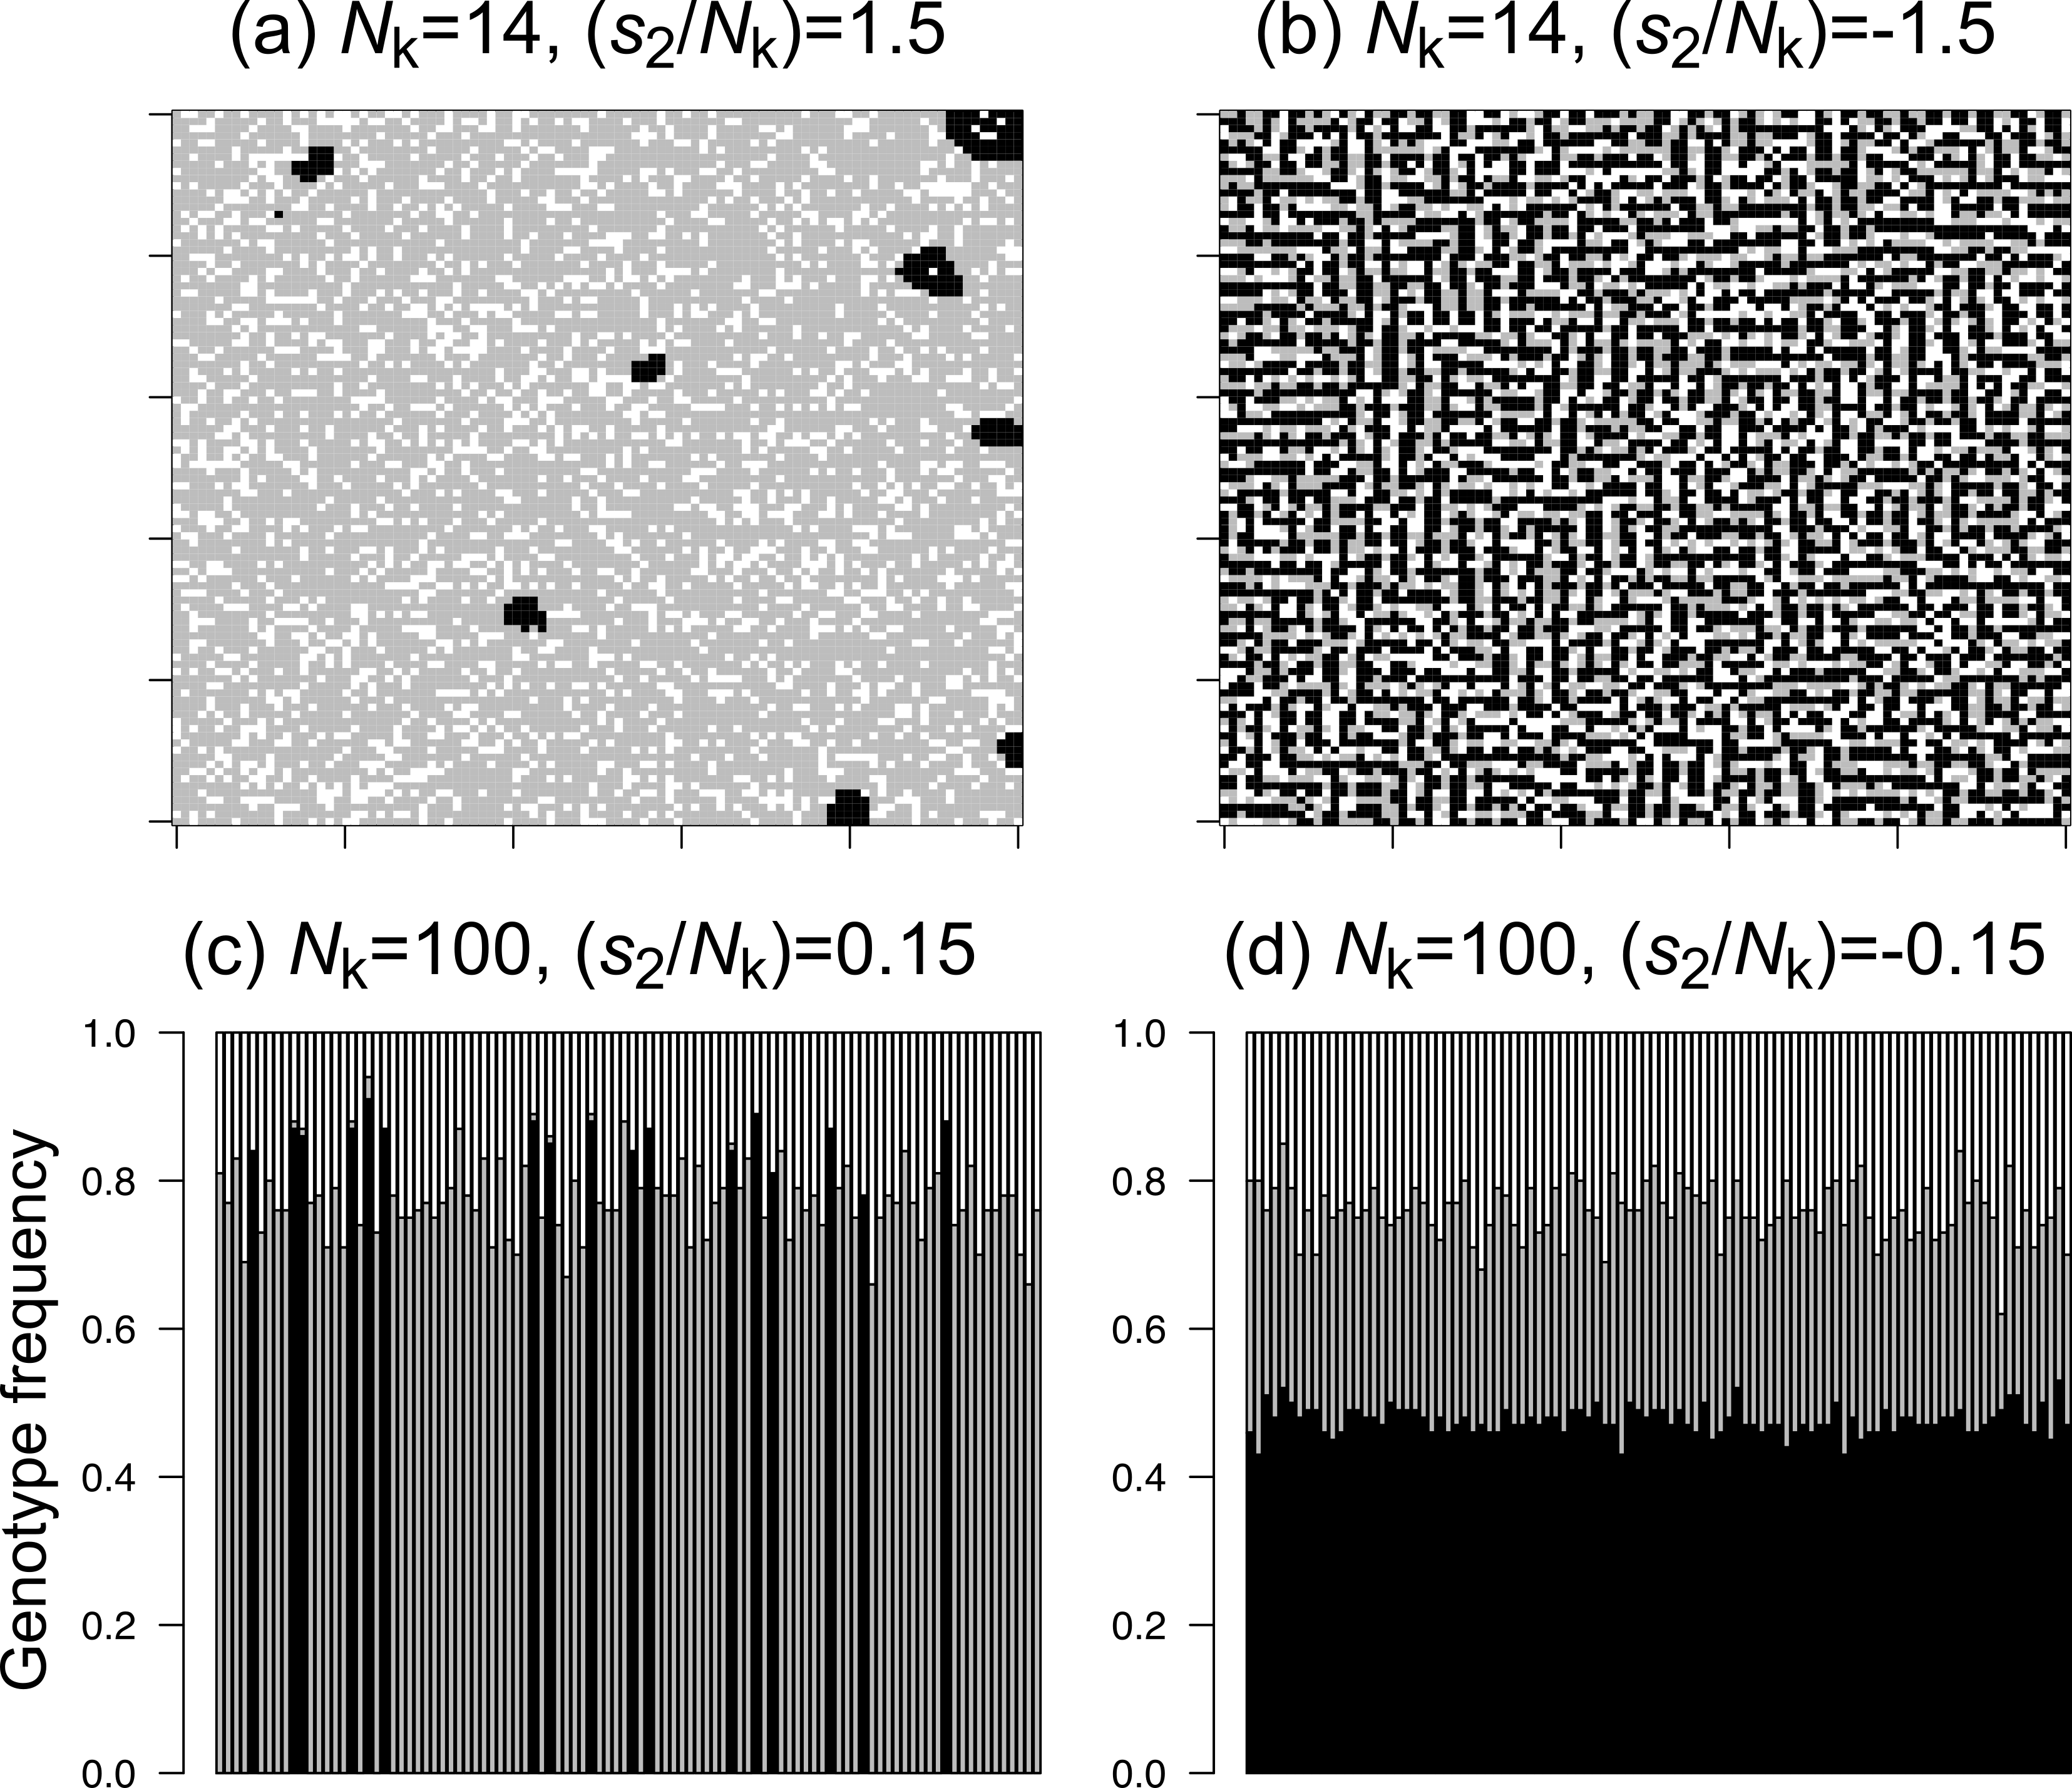
\includegraphics[width=0.8\linewidth]{IsingExample.png}
  \caption{Numerical simulations maximizing the fitness $w_1 = w_0 + s_1g_i + (s_2 / {N_k})\sum^{N_k}_{j=i}{g_ig_j}$ (Appendix S1) for 100 generations. White, gray, and black colors indicate the AA, Aa, and aa genotypes, respectively. The upper panels (a, b) represent plant genotype distributions across a 100 $\times$ 100 continuous lattice space when interactions are restricted to the second nearest neighbors ($N_k=14$). Each grid corresponds to an individual. Lower panels (c, d) represent the genotype frequencies among 100 split populations composed of 100 individuals each. Each vertical bar corresponds to a population. Left panels (a, c) simulate positive frequency-dependent selection (FDS), while right panels (b, d) simulate negative FDS. The base fitness and directional selection coefficient were set at $w_0 = 0$ and $s_1 = 10^{-4}$ for all simulations, while the subpopulation size $N_k$ and interaction strength per individual $s_2/N_k$ were changed.}
  \label{figS1:Ising}
\end{figure}

The probability of sampling AA, Aa, or aa at $t+1$ generation is denoted as $P_{\mathrm{AA},t+1}$, $P_{\mathrm{Aa},t+1}$, and $P_{\mathrm{aa},t+1}$, respectively. Let $f_\mathrm{AA}$, $f_\mathrm{Aa}$, and $f_\mathrm{aa}$ be the frequencies of genotypes AA, Aa, and aa within a population with $f_\mathrm{AA}$, $f_\mathrm{Aa}$, and $f_\mathrm{aa}$. In summary, the transition from generation $t$ to $t+1$ is expressed as:

$$
\left( \begin{array}{cc} 
    P_{\mathrm{AA},t+1}\\ 
    P_{\mathrm{Aa},t+1}\\
    P_{\mathrm{aa},t+1}\\
    \end{array} \right) 
    =
\left(\begin{array}{ccc}
    (f_\mathrm{AA}+0.5f_\mathrm{Aa}) & (0.5f_\mathrm{AA}+0.25f_\mathrm{Aa}) & 0\\ 
    (f_\mathrm{aa}+0.5f_\mathrm{Aa}) & (0.5f_\mathrm{AA}+0.5f_\mathrm{Aa}+0.5f_\mathrm{aa}) & (f_\mathrm{AA}+0.5f_\mathrm{Aa})\\
    0 & (0.25f_\mathrm{Aa}+0.5f_\mathrm{aa}) & (0.5f_\mathrm{Aa}+f_\mathrm{aa})\\
    \end{array} \right) 
\left( \begin{array}{cc} 
    P_{\mathrm{AA},t}\\ 
    P_{\mathrm{Aa},t}\\
    P_{\mathrm{aa},t}\\
    \end{array} \right),
$$
\noindent
where the elements of the transition matrix were calculated from the three genotype frequencies and the segregation ratio of Mendelian inheritance. The zero elements pose a constraint where one homozygote cannot turn into another homozygote in a single generation. Given that the sum of the three genotype frequencies was 1 as $f_\mathrm{AA}+f_\mathrm{Aa}+f_\mathrm{aa}=1$, the probability of staying as a heterozygote was 0.5. Therefore, the outcome from the modified Metropolis algorithm was expected to be qualitatively the same as a random proposal of three genotypes but quantitatively different in the excess of heterozygotes within a population.

Figure \ref{figS1:Ising} shows the results of the numerical simulations with the three genotypes encoded as $g_{i(j)} \in$ \{AA, Aa, aa\} $=$ \{+1, +1, -1\}. The three genotypes were well mixed and maintained in a continuous space when $s_2<0$ (Fig. \ref{figS1:Ising}b), whereas several clusters of the aa genotype were observed when $s_2>0$ (Fig. \ref{figS1:Ising}a). Three genotypes were also maintained at an intermediate frequency in a split space when $s_2<0$ (Fig. \ref{figS1:Ising}d), whereas the allele frequency was heavily biased when $s_2>0$ (Fig. \ref{figS1:Ising}c). The numerical simulations show that the sign of $s_2$ likely corresponded to the direction of the frequency-dependent selection (FDS) in a continuous and split space.

\medskip
\subsection*{Appendix S2. Mixed model extension}
To implement GWAS, we modified Equations (\ref{eq:2}) and (\ref{eq:3}) as a linear mixed model (LMM) that considered genetic relatedness as a random effect \citep{kang2008efficient}. In terms of Henderson's mixed model \citep{henderson1959estimation}, such GWAS models have the same structure as phylogenetic comparative methods that analyze interspecific phenotypic variation among phylogenetic trees \citep{kang2008efficient, hadfield2010general}. According to \cite{hadfield2010general}, we designated the genetic-related matrix as $\mathbf{A}$ and introduced random effects $u_i$ to Equation (\ref{eq:2}) as follows: 

\begin{equation}
y_i = \beta_0 + \beta_1x_i + \beta_2\sum^{N_{k}}_{j=1}{x_ix_j} + u_i + e_i \label{eq:s1}
\end{equation}
\noindent
where a vector including $u_i$ for $n$ individuals followed a normal distribution as $u_i \in \mathbf{u}$ and $\mathbf{u} \sim$ Norm($\mathbf{0}$, $\sigma^2_1\mathbf{A}_1+\sigma^2_2\mathbf{A}_2$). The residual $e_i$ is expressed as $e_i \in \mathbf{e}$ and $\mathbf{e} \sim$ Norm($\mathbf{0}$, $\sigma^2_e\mathbf{I}$).
The $n$ × $n$ variance-covariance matrices denote the self-genetic relatedness or the entire genotype similarity among $n$ individuals as
$\mathbf{A}_1=\frac{1}{2(q-1)}\mathbf{X}_1^\mathsf{T}\mathbf{X}_1 + \frac{1}{2}$ and 
$\mathbf{A}_2=\frac{1}{(q-1)}\mathbf{X}_2^\mathsf{T} \mathbf{X}_2$
where $q$ denotes the number of loci. The elements of $n$ individuals $\times$ $q$ loci matrix $\mathbf{X}_1$ consist of explanatory variables of the self-genotype values. As we defined $x_{i(j)} = (-1, 1)$, the genetic-related matrix $\mathbf{A}_1$ was scaled to represent the proportion of loci shared among $n$ × $n$ individuals. The elements of $n$ individuals $\times$ $q$ loci matrix $\mathbf{X}_2$ consist of the genotype similarity as:

$$\mathbf{X}_2=\left(\begin{array}{cccc}
    (\sum^{N_k}_{j=1}x_{1,1} x_j)/N_k &  (\sum^{N_k}_{j=1}x_{1,2} x_j)/N_k &  ... &  (\sum^{N_k}_{j=1}x_{1,n} x_j)/N_k \\ 
    (\sum^{N_k}_{j=1}x_{1,2} x_j)/N_k &  (\sum^{N_k}_{j=1}x_{2,2} x_j)/N_k &  ... &  (\sum^{N_k}_{j=1}x_{2,n} x_j)/N_k\\
    ... & ... & ... & ... \\
    (\sum^{N_k}_{j=1}x_{q,1} x_j)/N_k &  (\sum^{N_k}_{j=1}x_{q,2} x_j)/N_k &  ... &  (\sum^{N_k}_{j=1}x_{q,n} x_j)/N_k \\
    \end{array} \right)
$$,
where the $n \times n$ matrix $\mathbf{A}_2$ indicates a sample structure related to genotype similarity. The variance component parameters $\sigma^2_1$ and $\sigma^2_2$ determine the relative contributions of $\mathbf{A}_1$ and $\mathbf{A}_2$ to the vector of random effects $\mathbf{u}$.

To incorporate asymmetric FDS into GWAS, we considered a sample structure based on the asymmetric FDS in LMM. Here, we extended Equation (\ref{eq:3}) into LMM as:

\begin{equation}
y_i = \beta_0 + \beta_1x_i + \frac{\beta_2}{N_k}\sum^{N_{k}}_{j=1}{x_ix_j} + \frac{\beta_{12}x_i}{N_k}\sum^{N_{k}}_{j=1}{x_ix_j} + u_i + e_i \label{eq:s2}
\end{equation}
\noindent
where the random effect $u_i$ is redefined as $u_i \in \mathbf{u}$ and $\mathbf{u} \sim$ Norm($\mathbf{0}$, $\sigma^2_1\mathbf{A}_1+\sigma^2_2\mathbf{A}_2+\sigma^2_{12}\mathbf{A}_{12}$). The additional $n \times n$ variance-covariance matrix $\mathbf{A}_{12}$ denotes a sample structure because of the asymmetric effects among $n$ individuals as $\mathbf{A}_{12}=\frac{1}{(q-1)}\mathbf{X}_{12}^\mathsf{T} \mathbf{X}_{12}$. The elements of $n$ individuals $\times$ $q$ loci matrix $\mathbf{X}_{12}$ consist of explanatory variables for the asymmetric effects as follows:

$$\mathbf{X}_{12}=\left(\begin{array}{cccc}
    (x_{1,1}\sum^{N_k}_{j=1}x_{1,1} x_j)/N_k &  (x_{1,2}\sum^{N_k}_{j=1}x_{1,2} x_j)/N_k &  ... &  (x_{1,n}\sum^{N_k}_{j=1}x_{1,n} x_j)/N_k \\ 
    (x_{1,2}\sum^{N_k}_{j=1}x_{1,2} x_j)/N_k &  (x_{2,2}\sum^{N_k}_{j=1}x_{2,2} x_j)/N_k &  ... &  (x_{2,n}\sum^{N_k}_{j=1}x_{2,n} x_j)/N_k\\
    ... & ... & ... & ... \\
    (x_{q,1}\sum^{N_k}_{j=1}x_{q,1} x_j)/N_k &  (x_{q,2}\sum^{N_k}_{j=1}x_{q,2} x_j)/N_k &  ... &  (x_{q,n}\sum^{N_k}_{j=1}x_{q,n} x_j)/N_k \\
    \end{array} \right)
$$
The additional parameter of the variance component $\sigma^2_{12}$ compares the relative importance of the asymmetric effects with those of the self-genotype effects $\sigma^2_1$ and genotype similarity effects $\sigma^2_2$.
In addition, the individual-level formula Equation (\ref{eq:s1}) can also be converted into a common matrix form \citep{henderson1959estimation} as:

\begin{equation}
    \mathbf{y}=\mathbf{X}\bm{\beta}+\mathbf{Zu}+\mathbf{e} \label{eq:s3}
\end{equation}

where $\mathbf{y}$ is $n \times 1$ fitness vector with $y_i \in \mathbf{y}$; $\mathbf{X}$ is a matrix of fixed effects, including a unit vector, self-genotype $x_i$, genotype similarity covariate $(\sum^{N_k}_{j=1}x_i x_j)/N_k$, and other covariates for $n$ individuals; $\bm{\beta}$ is a vector that included coefficients of the fixed effects; $\mathbf{Z}$ is a design matrix allocating individuals to a genotype; $\mathbf{u}$ is the random effect as Var($\mathbf{u}$) $=\sigma^2_1\mathbf{A}_1+\sigma^2_2\mathbf{A}_2+\sigma^2_{12}\mathbf{A}_{12}$; and $\mathbf{e}$ is the residual as Var($\mathbf{e}$) $=\sigma^2_e\mathbf{I}$. 

To efficiently solve LMMs, we first estimated $\sigma^2_1$ and $\sigma^2_2$ without any fixed effects (i.e., null model) using the average-information restricted maximum likelihood method implemented in the gaston package \citep{R_gaston}. Then, to compare the significance of $\beta_1$ and $\beta_2$ to the null model, we solved Equation (\ref{eq:s3}) using fast approximation by eigenvalue decomposition on a random effect matrix $\hat{\sigma}^2_1\mathbf{A}_1+\hat{\sigma}^2_2\mathbf{A}_2+\hat{\sigma}^2_{12}\mathbf{A}_{12}$. The likelihood ratio test was used to compare the models with and without $\beta_2$. The standard GWAS is a subset of Equation (\ref{eq:s1}) when $\beta_2=0$ and $\sigma^2_2=0$ \citep{sato2019neighbor}; thus, we set $\beta_2$ and $\sigma^2_2$ to zero when testing $\beta_1$. Such stepwise likelihood ratio tests were essential for conservative tests of each parameter in Equations (\ref{eq:s1}) and (\ref{eq:s2}), because the self-genotype variable $x_i$ and the genotype similarity variable $(\sum^{N_{k}}_{j=1}{x_ix_j})/N_k$ were strongly correlated when the MAF was very small \citep{sato2019neighbor}. Stepwise likelihood ratio tests were implemented using the rNeighborGWAS package version 1.2.4 \citep{sato2019neighbor}. The nei\_lmm() function was applied for power analysis and GWAS in the main text. The "asym = TRUE" option was chosen when testing the asymmetric effects $\beta_{12}$.


\medskip
\subsection*{Appendix S3. Fitness function under symmetric and asymmetric FDSs}
To analyze the regression model Equation (\ref{eq:3}) as a fitness function of allele frequency, we considered a single diallelic locus in an ideal population where (i) diploid individuals were randomly mating, (ii) uniformly interacting, and (iii) the population size was sufficiently large (i.e., $N \to \infty$). We also assumed no maternal or paternal effects on fitness, such that the genotypes Aa and aA could not be distinguished. To concentrate on the mean trends of the model, we neglected the residuals as $e_i = 0$. Replacing $N_{k}$ into $N$, we redefined Equation (\ref{eq:3}) as follows:

\begin{equation}
y_i = \beta_0 + \beta_1x_i + \frac{\beta_2}{N}\sum^{N}_{j=1}{x_ix_j} + \frac{\beta_{12}x_i}{N}\sum^{N}_{j=1}{x_ix_j} \label{eq:s4}
\end{equation}
\noindent
where the trait value $y_i$ corresponds to the fitness value $w_i$ for individual $i$, the intercept $\beta_0$ corresponds to the base fitness $w_0$, the self-genotype coefficient $\beta_1$ corresponds to the directional selection coefficient $s_1$, and the coefficients $\beta_2$ and $\beta_{12}$ correspond to the selection coefficients related to FDS. The second term can also be transformed for simplicity as $\beta_2(\sum^{N}_{j=1}x_i x_j)/N = \beta_2x_i(\sum^{N}_{j=1}x_j)/N$, and the third term, $\beta_{12}x_i(\sum^{N}_{j=1}x_i x_j)/N = \beta_{12}x^2_i(\sum^{N}_{j=1}x_j)/N$. Provided $x^2_i=(-1)^2=1^2=1$, the third term represents a selection gradient due to the relative abundance of one allele in a neighborhood, irrespective of the self-genotype of a focal individual $i$.

We then transformed Equation (\ref{eq:s4}) into a function of the frequency of A alleles $f$, where the frequency of an allele was defined conversely as $1-f$. When all the individuals were randomly interacting in a panmictic population, the interaction strength between $i$ and $j$ depended on the frequencies of AA, Aa, or aa genotypes derived from allele frequency. Thus, the fitness values of the three genotypes, $y_\mathrm{AA}(f)$, $y_\mathrm{Aa}(f)$, and $y_\mathrm{aa}(f)$, are functions of allele frequency $f$. For convenience, we suppressed the dependence on $f$, unless necessary. The ratio of AA, Aa, and aa genotypes within the panmictic population was given by AA:Aa:aa $=f^2: 2f(1-f)$: $(1-f)^2$. Assuming the aforementioned ideal population, we designated all combinations of interactions among AA, Aa, and aa genotypes and weighted the interactions based on their genotype frequencies. Table \ref{tableS2:intTable} lists the interaction strength weighted by the genotype frequency for symmetric and asymmetric effects. Based on these cross tables (Table \ref{tableS2:intTable}), we redefined Equation (\ref{eq:s4}) for the three genotypes as: 

\begin{table}[h]
\caption{Cross tables showing the strength of pairwise interactions between the focal genotype $x_i$ and counterpart $x_j$ in a randomly interacting and mating population.}
(a) Symmetric effects \\
\begin{tabular}{|l|lll|}
\hline
$x_j$ \textbackslash{} $x_i$ & $x_\mathrm{AA}$ & $x_\mathrm{Aa}$ & $x_\mathrm{aa}$ \\ \hline
$x_\mathrm{AA}$ & $\beta_2 f^2x_\mathrm{AA}x_\mathrm{AA}$ & $\beta_2f^2x_\mathrm{Aa}x_\mathrm{AA}$ & $\beta_2f^2x_\mathrm{aa}x_\mathrm{AA}$ \\
$x_\mathrm{Aa}$ & $2\beta_2f(1-f)x_\mathrm{AA}x_\mathrm{Aa}$ & $2\beta_2f(1-f)x_\mathrm{Aa}x_\mathrm{Aa}$ & $2\beta_2f(1-f)x_\mathrm{aa}x_\mathrm{Aa}$ \\
$x_\mathrm{aa}$ & $\beta_2(1-f)^2x_\mathrm{AA}x_\mathrm{aa}$ & $\beta_2(1-f)^2x_\mathrm{Aa}x_\mathrm{aa}$ & $\beta_2(1-f)^2x_\mathrm{aa}x_\mathrm{aa}$ \\ \hline
\end{tabular}

\vspace*{5mm}

(b) Asymmetric effects \\
\begin{tabular}{|l|lll|}
\hline
$x_j$ \textbackslash{} $x_i$ & $x_\mathrm{AA}$ & $x_\mathrm{Aa}$ & $x_\mathrm{aa}$ \\ \hline
$x_\mathrm{AA}$ & $\beta_{12}f^2x^2_\mathrm{AA}x_\mathrm{AA}$  &  $\beta_{12}f^2x^2_\mathrm{Aa}x_\mathrm{AA}$  & $\beta_{12}f^2x^2_\mathrm{aa}x_\mathrm{AA}$ \\
$x_\mathrm{Aa}$ & $2\beta_{12}f(1-f)x^2_\mathrm{AA}x_\mathrm{Aa}$ & $2\beta_{12}f(1-f)x^2_\mathrm{Aa}x_\mathrm{Aa}$ &  $2\beta_{12}f(1-f)x^2_\mathrm{aa}x_\mathrm{Aa}$ \\
$x_\mathrm{aa}$ & $\beta_{12}(1-f)^2x^2_\mathrm{AA}x_\mathrm{aa}$ & $\beta_{12}(1-f)^2x^2_\mathrm{Aa}x_\mathrm{aa}$ & $\beta_{12}(1-f)^2x^2_\mathrm{aa}x_\mathrm{aa}$ \\ \hline
\end{tabular}
      \label{tableS2:intTable}
\end{table}

\begin{subequations} \label{eq:s5}
\begin{gather}
    \begin{split}
y_\mathrm{AA} &= \beta_0 + \beta_1x_\mathrm{AA} + \beta_2f^2x_\mathrm{AA}x_\mathrm{AA} + 2\beta_2f(1-f)x_\mathrm{AA}x_\mathrm{Aa} + \beta_2(1-f)^2x_\mathrm{AA}x_\mathrm{aa} \\
& + \beta_{12}f^2x^2_\mathrm{AA}x_\mathrm{AA} + 2\beta_{12}f(1-f)x^2_\mathrm{AA}x_\mathrm{Aa}+ \beta_{12}(1-f)^2x^2_\mathrm{AA}x_\mathrm{aa} \label{eq:s5a}
    \end{split}
\end{gather}
\begin{gather}
    \begin{split}
y_\mathrm{Aa} &= \beta_0 + \beta_1x_\mathrm{Aa} + \beta_2f^2x_\mathrm{Aa}x_\mathrm{AA} + 2\beta_2f(1-f)x_\mathrm{Aa}x_\mathrm{Aa} + \beta_2(1-f)^2x_\mathrm{Aa}x_\mathrm{aa} \\
& + \beta_{12}f^2x^2_\mathrm{Aa}x_\mathrm{AA} + 2\beta_2f(1-f)x^2_\mathrm{Aa}x_\mathrm{Aa}+ \beta_{12}(1-f)^2x^2_\mathrm{Aa}x_\mathrm{aa} \label{eq:s5b}
    \end{split}
\end{gather}
\begin{gather}
    \begin{split}
y_\mathrm{aa} &= \beta_0 + \beta_1x_\mathrm{aa} + \beta_2f^2x_\mathrm{aa}x_\mathrm{AA} + 2\beta_2f(1-f)x_\mathrm{aa}x_\mathrm{Aa} + \beta_2(1-f)^2x_\mathrm{aa}x_\mathrm{aa} \\
& + \beta_{12}f^2 x^2_\mathrm{aa}x_\mathrm{AA} + 2\beta_2f(1-f)x^2_\mathrm{aa}x_\mathrm{Aa}+ \beta_{12}(1-f)^2x^2_\mathrm{aa}x_\mathrm{aa} \label{eq:s5c}
    \end{split}
\end{gather}
\end{subequations}

\noindent
We further weighted the genotype-level fitness values by allele frequency. The allele-level marginal fitness for A or an allele is then given by:

\begin{subequations} \label{eq:s6}
\begin{align}
y_\mathrm{A} = fy_\mathrm{AA} + (1-f)y_\mathrm{Aa} \label{eq:s6a} \\
y_\mathrm{a} = fy_\mathrm{Aa} + (1-f)y_\mathrm{aa} \label{eq:s6b}
\end{align}
\end{subequations}

\noindent
The population-level mean fitness was finally defined by the weighted mean of the marginal fitness as follows:

\begin{equation}
\begin{split}
\bar{y} &= fy_\mathrm{A} + (1-f)y_\mathrm{a} \\
&= f^2y_\mathrm{AA} + 2f(1-f)y_\mathrm{Aa} + (1-f)^2y_\mathrm{aa} \label{eq:s7}
\end{split}
\end{equation}

\noindent
Consequently, we could analyze fitness functions by inputting specific values in the three genotype values $x_\mathrm{AA}, x_\mathrm{Aa}$, and $x_\mathrm{aa}$ throughout Equations (\ref{eq:s5}) and (\ref{eq:s6}).

Case 1. Complete dominance with random mating: Novel mutations are expected to be recessive during adaptive evolution. Empirical studies have reported FDS on dimorphic traits that often exhibit complete dominance of one over another allele \citep[e.g.,][]{takahashi2010negative,sato2017herbivore,goldberg2020herbivore}. First, we considered the case in which the A allele was completely dominant over an allele, as encoded by $x_{i(j)} \in$ \{AA, Aa, aa\} $=$ \{+1, +1, -1\}. Here, we neglected the directional selection as $\beta_1=0$ in Equation (\ref{eq:s5}) to focus on the fitness functions under FDS alone. Replacing the genotypes ($x_\mathrm{AA}$, $x_\mathrm{Aa}$, and $x_\mathrm{aa}$) according to their genotype values in Equation (\ref{eq:s5}) gave the fitness value to the three genotypes as:

\begin{subequations}
\begin{gather}
    \begin{split}
y_\mathrm{AA} = y_\mathrm{Aa} &= \beta_0 + \beta_2 [(+1)\times(+1)] f^2 + \beta_2 [(+1)\times(+1)] 2f(1-f) + \beta_2 [(+1)\times(-1)] (1-f)^2 \\
& + \beta_{12} [(+1)^2\times(+1)] f^2 + \beta_{12} [(+1)^2\times(+1)] 2f(1-f) + \beta_{12} [(+1)^2\times(-1)] (1-f)^2 \\ 
&= \beta_0 + \beta_2(2f-1+2f-2f^2) + \beta_{12}(2f-1+2f-2f^2) \\
&= \beta_0 + (\beta_{12}+\beta_2)(4f-2f^2-1)~~~\mathrm{where}~x_\mathrm{AA}=x_\mathrm{Aa} = +1 \label{eq:s8a}
    \end{split}
\end{gather}
\begin{gather}
    \begin{split}
y_\mathrm{aa} &= \beta_0 + \beta_2[(-1)\times(+1)]f^2 + \beta_2[(-1)\times(+1)]2f(1-f) + \beta_2[(-1)\times(-1)](1-f)^2 \\
& + \beta_{12}[(-1)^2\times(+1)]f^2 + \beta_{12}[(-1)^2\times(+1)]2f(1-f) + \beta_{12}[(-1)^2\times(-1)](1-f)^2 \\ 
&= \beta_0 - \beta_2(2f-1+2f-2f^2) + \beta_{12}(2f-1+2f-2f^2) \\
&= \beta_0 + (\beta_{12}-\beta_2)(4f-2f^2-1)~~~\mathrm{where}~x_\mathrm{aa} = +1 \label{eq:s8b}
    \end{split}
\end{gather}
\end{subequations}

\noindent
The marginal fitness following Equations (\ref{eq:s6a}) and (\ref{eq:s6b}) was given by 

\begin{subequations}
\begin{align}
y_\mathrm{A} = fy_\mathrm{AA} + (1-f)y_\mathrm{Aa} = fy_\mathrm{AA} + (1-f)y_\mathrm{AA} = y_\mathrm{AA} \label{eq:s9a} \\
y_\mathrm{a} = fy_\mathrm{Aa} + (1-f)y_\mathrm{aa} = y_\mathrm{aa} + 2f\beta_2(4f-2f^2-1) \label{eq:s9b}
\end{align}
\end{subequations}

\noindent
The relative fitness between A and a alleles was calculated as: $y_\mathrm{A} - y_\mathrm{a} = y_\mathrm{AA} - y_\mathrm{aa} - 2f\beta_2(4f-2f^2-1) = 2\beta_2(1-f)(4f-2f^2-1)$. Solving $y_\mathrm{A} - y_\mathrm{a} = 0$ with respect to $f$ within the range of (0,1) resulted in $f^*=-0.5\sqrt{2}+1$, which showed a single stable or unstable state within $f=(0,1)$ in the case of complete dominance under FDS. The population-level mean fitness is finally given by:

\begin{equation}
\begin{split}
\bar{y} &= fy_\mathrm{A} + (1-f)y_\mathrm{a} \\
&= \beta_0 + (4f\beta_2-2f^2\beta_2-\beta_2+\beta_{12})(4f-2f^2-1) \label{eq:s10}
\end{split}
\end{equation}

\noindent
Figure \ref{fig2:asym} in the main text shows the marginal fitness [Equations (\ref{eq:s9a}) and (\ref{eq:s9b})] and mean fitness [Equation (\ref{eq:s10})]. The mean fitness was maximized at a stable equilibrium at the intermediate allele frequency under symmetric negative FDS, whereas it was minimized at an unstable equilibrium under symmetric positive FDS. When asymmetric FDS and complete dominance are involved, equilibria do not always match the maxima or minima of the mean fitness because of the nonlinearity of the marginal fitness in response to $f$. However, the mean fitness at the stable or unstable point was still higher or lower than expected compared with the weighted mean of the two monomorphic populations. A similar notion was suggested by pairwise interaction models in population genetics \citep{cockerham1972frequency, schneider_maximization_2008}.

Case 2. Additive effects with random mating: Although few empirical studies have reported FDS on quantitative traits, this case is of theoretical interest in the pairwise interaction model \citep{schneider_maximization_2008}. Considering the fitness value as a quantitative trait, we then analyzed the additive effects of A and a alleles on $y_i$ as encoded by $x_{i(j)} \in $ \{AA, Aa, aa\} $=$ \{+1, 0, -1\}. Replacing the genotypes ($x_\mathrm{AA}$, $x_\mathrm{Aa}$, and $x_\mathrm{aa}$) according to their genotype values in Equations (\ref{eq:s5}) gave the fitness value to the three genotypes as:

\begin{subequations}
\begin{gather}
    \begin{split}
y_\mathrm{AA} &= \beta_0 + \beta_2 [(+1)\times(+1)] f^2 + \beta_2 [(+1)\times(-1)] (1-f)^2 \\
& + \beta_{12} [(+1)^2\times(+1)] f^2 + \beta_{12} [(+1)^2\times(-1)] (1-f)^2 \\ 
&= \beta_0 + \beta_2f^2 - \beta_2(1-2f+f^2) + \beta_{12}f^2 - \beta_{12}(1-2f+f^2) \\
&= \beta_0 + \beta_2(2f - 1) + \beta_{12}(2f-1) \\ 
&= \beta_0 + (\beta_{12}+\beta_2)(2f-1)~~~\mathrm{where}~x_\mathrm{AA} = +1 \label{eq:s11a}
    \end{split}
\end{gather}
\begin{gather}
    y_\mathrm{Aa} = \beta_0~~~\mathrm{where}~x_\mathrm{Aa} = 0 \label{eq:s11b}
\end{gather}
\begin{gather}
    \begin{split}
y_\mathrm{aa} &= \beta_0 + \beta_2 [(-1)\times(+1)] f^2\ + \beta_2 [(-1)\times(+1)] (1-f)^2 \\
& + \beta_{12} [(-1)^2\times(+1)] f^2 + \beta_{12} [(-1)^2\times(-1)] (1-f)^2 \\
&= \beta_0 - \beta_2f^2 + \beta_2(1-2f+f^2) + \beta_{12}f^2 - \beta_{12}(1-2f+f^2) \\
&= \beta_0 - \beta_2(2f - 1) + \beta_{12}(2f-1) \\
&= \beta_0 + (\beta_{12} - \beta_2)(2f - 1)~~~\mathrm{where}~x_\mathrm{aa} = -1 \label{eq:s11c}
    \end{split}
\end{gather}
\end{subequations}

\noindent
The fitness function for the two homozygotes AA and aa [i.e., Equations (\ref{eq:s5a}) and (\ref{eq:s5c})] turned out to be linear in response to $f$. The marginal fitness following Equations (\ref{eq:s6a}) and (\ref{eq:s6b}) is then given by:

\begin{subequations}
\begin{gather}
    \begin{split}
y_\mathrm{A} &= fy_\mathrm{AA} + (1-f)y_\mathrm{Aa}\\
&= \beta_0+f(\beta_{12}+\beta_2)(2f-1) \label{eq:s12a}
    \end{split}
\end{gather}
\begin{gather}
    \begin{split}
y_\mathrm{a} &= fy_\mathrm{Aa} + (1-f)y_\mathrm{aa}\\
&= \beta_0+(1-f)(\beta_{12}-\beta_2)(2f-1) \label{eq:s12b}
    \end{split}
\end{gather}
\end{subequations}

\noindent
The relative fitness was calculated as $y_\mathrm{A} - y_\mathrm{a} = (2f-1)[f(\beta_{12}+\beta_2) - (1-f)(\beta_{12}-\beta_2)] = (2f-1)(2\beta_{12}f-\beta_{12}+\beta_2)$. Solving $y_\mathrm{A} - y_\mathrm{a} = 0$ with respect to $f$ within a range of (0,1) yields $f^*=0.5$ and $f^*=0.5(\beta_{12}-\beta_2)/\beta_{12}$, showing that the additive action of FDS made multiple equilibria possible at the intermediate allele frequency $f = (0,1)$. The mean fitness following Equation (\ref{eq:s7}) is finally given by:

\begin{equation}
\begin{split}
\bar{y} &= fy_\mathrm{A} + (1-f)y_\mathrm{a} \\
&= \beta_0 + f^2(\beta_{12}+\beta_2)(2f-1) + (1-f)^2(\beta_{12}-\beta_2)(2f-1)\\
&= \beta_0 + (2f-1)[2f^2(\beta_{12}+\beta_2)-2f(\beta_{12}-\beta_2)+\beta_{12}-\beta_2] \label{eq:s13}
\end{split}
\end{equation}

\noindent
Figure \ref{figS2:FDSadd} shows numerical examples of the marginal fitness [Equations (\ref{eq:s12a}) and (\ref{eq:s12b})] and the mean fitness [Equation (\ref{eq:s13})] in response to $f$. Similar to the case of complete dominance, the mean fitness was maximized or minimized at a stable or unstable equilibrium under the symmetric FDS (Fig. \ref{figS2:FDSadd}a and b). In contrast, a stable and unstable equilibrium occurred simultaneously under asymmetric FDS (Fig. \ref{figS2:FDSadd}c and f), where the maxima or minima of mean fitness did not always match the equilibria. This potential of multiple equilibria was also suggested by a one-locus two-allele model of pairwise interactions when it involved asymmetric FDS \citep{schneider_maximization_2008}. 

\begin{figure}[]
  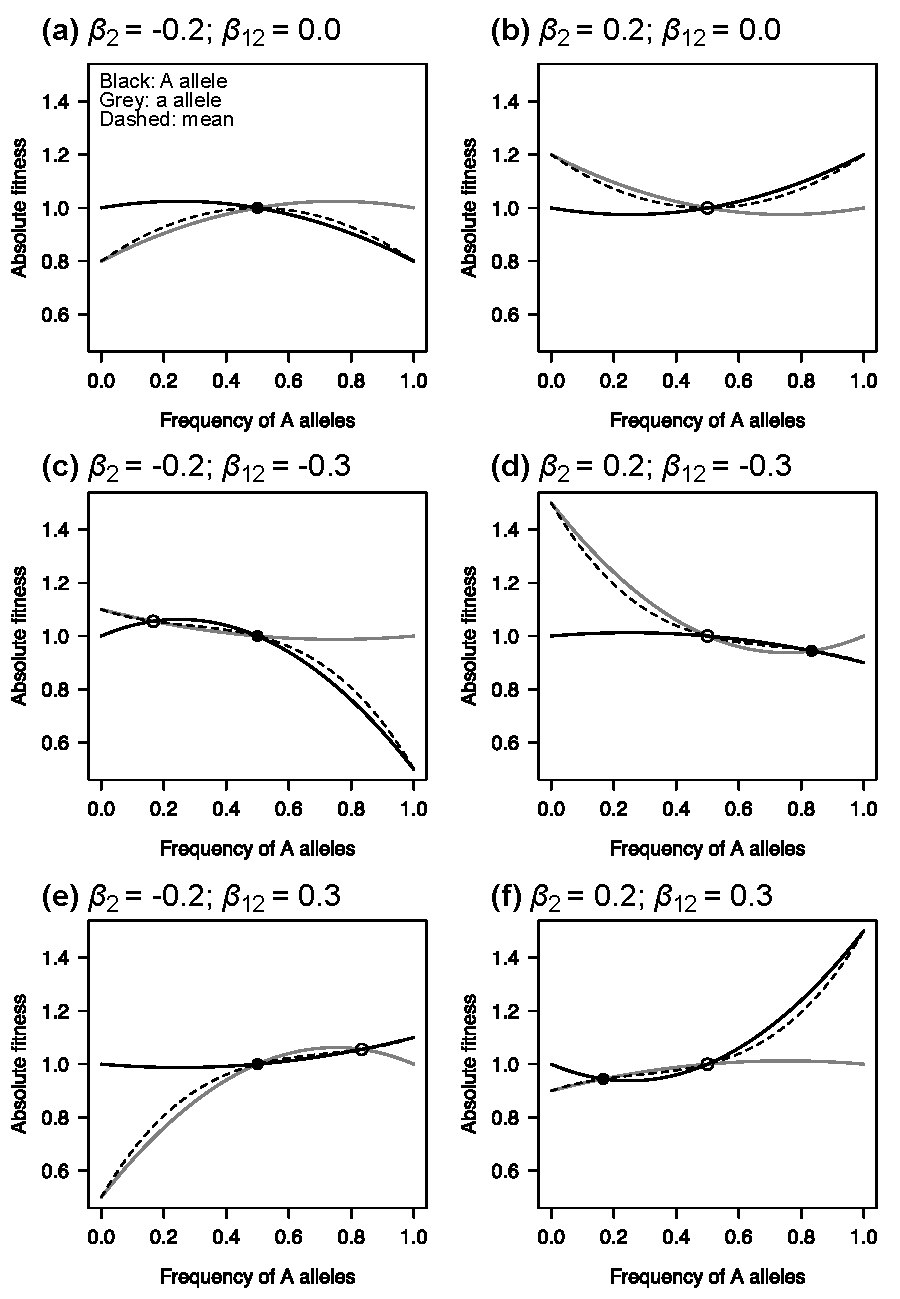
\includegraphics[width=0.7\linewidth]{AsymFDSadd.pdf}
  \caption{Numerical examples for the fitness values $y_i$ in response to allele frequency when A and a alleles have additive effects on the fitness; that is, Equations (\ref{eq:s12a}) and (\ref{eq:s12b}) in Appendix S3. Black and gray lines indicate the marginal fitness of the A allele or an allele, respectively. The dashed curves indicate the mean fitness per population; that is, Equation (\ref{eq:s13}) in Appendix S3. (a) Symmetric negative frequency-dependent selection (FDS); (b) symmetric positive FDS; (c and e) asymmetric negative FDS; and (d and f) asymmetric positive FDS. Closed and open circles indicate a stable or unstable state, respectively. The base fitness and no directional selection were set at $\beta_0=1.0$ and $\beta_1=0.0$ for all panels.}
  \label{figS2:FDSadd}
\end{figure}

Case 3. Asexual or inbred lines without mating: In common gardens or laboratory experiments, researchers arbitrarily distribute inbred accessions in space and retrieve individuals before mating \citep[e.g.,][]{schutz1969inter, sato2019neighbor}. This was also the case for the field GWAS in the main text. Furthermore, ecological studies often focus on FDS at the phenotype level with asexual reproduction assumed \citep[e.g.,][]{takahashi2018balanced}. In these cases, heterozygosity was negligible, and the two homozygotes were encoded as $x_{i(j)} \in $ \{AA, aa\} $=$ \{+1, -1\} \citep{sato2019neighbor}. Let $f_\mathrm{AA}$ and $f_\mathrm{aa}$ be the frequency of AA and aa genotypes within a population, where $f_\mathrm{AA} + f_\mathrm{aa} = 1$. The fitness function for the AA or aa genotype is given by:

\begin{subequations}
\begin{gather}
    \begin{split}
y_\mathrm{AA} &= \beta_0 + \beta_2f_\mathrm{AA}[(+1)\times(+1)] + \beta_2(1-f_\mathrm{AA})[(+1)\times(-1)] \\
&+ \beta_{12}f_\mathrm{AA}[(+1)^2\times(+1)] + \beta_{12}(1-f_\mathrm{AA})[(+1)^2\times(-1)] \\ 
&= \beta_0 + \beta_2(2f_\mathrm{AA}-1) + \beta_{12}(2f_\mathrm{AA}-1) \\ 
&= \beta_0 + (\beta_{12}+\beta_2)(2f_\mathrm{AA}-1)~~~\mathrm{where}~x_\mathrm{AA} = +1 \label{eq:s14a}
    \end{split}
\end{gather}
\begin{gather}
    \begin{split}
y_\mathrm{aa} &= \beta_0 + \beta_2f_\mathrm{AA}[(-1)\times(+1)] + \beta_2(1-f_\mathrm{AA})[\times(-1)\times(-1)] \\
&+ \beta_{12}f_\mathrm{AA}[(-1)^2\times(+1) + \beta_{12}(1-f_\mathrm{AA})[(-1)^2\times(-1)] \\
&= \beta_0 - \beta_2(2f_\mathrm{AA}-1) + \beta_{12}(2f_\mathrm{AA}-1) \\
&= \beta_0 + (\beta_{12}-\beta_2)(2f_\mathrm{AA}-1)~~~\mathrm{where}~x_\mathrm{aa} = -1 \label{eq:s14b}
    \end{split}
\end{gather}
\end{subequations}

\noindent
where the population-level mean fitness was given by its weighted mean as follows. 

\begin{equation}
\begin{split}
\bar{y} &= f_\mathrm{AA}y_\mathrm{AA} + (1-f_\mathrm{AA})y_\mathrm{aa} \\
&= f_\mathrm{AA}(y_\mathrm{AA}-y_\mathrm{aa}) + y_\mathrm{aa} \\
&= 2\beta_{2}f_\mathrm{AA}(2f_\mathrm{AA}-1) + (\beta_{12}-\beta_2)(2f_\mathrm{AA}-1) + \beta_0 \label{eq:s15}
\end{split}
\end{equation}

Figure \ref{figS3:FDSinbred} shows the fitness function of the AA or aa genotype [Equations (\ref{eq:s14a}) and (\ref{eq:s14b})] and population mean [Equation \ref{eq:s15}]. The fitness function of the two homozygotes was the same as that of the additive case described above. The mean fitness became simpler as the allele frequency corresponded to the genotype frequency. As this inbred case represented two genotypes with asexual reproduction, its conclusion was basically the same as that derived from game theoretical models \citep{takahashi2018balanced}. 

In Figure \ref{fig3:GLMM}, we present this inbred case with $\beta_1 \neq 0$, where the genotype fitness Equations (\ref{eq:s14a}) and (\ref{eq:s14b}) is rewritten as

\begin{subequations}
\begin{align}
    y_\mathrm{AA} = \beta_0 + \beta_1 + (\beta_{12}+\beta_2)(2f_\mathrm{AA}-1) \label{eq:s16a} \\
    y_\mathrm{aa} = \beta_0 - \beta_1 + (\beta_{12}-\beta_2)(2f_\mathrm{AA}-1) \label{eq:s16b}
\end{align}
\end{subequations}

\noindent
where the relative fitness is given by $y_\mathrm{AA} - y_\mathrm{aa} = 2\beta_1 + 2\beta_2(2f_\mathrm{AA}-1)$. Solving $y_\mathrm{AA} - y_\mathrm{aa} = 0$ with respect to $f_\mathrm{AA} = (0,1)$ yields $f^*_\mathrm{AA} = 1 - 0.5\beta_1 / \beta_2$. Therefore, the directional selection coefficient $\beta_1$ may modify the equilibrium. When $\beta_1 \neq 0$, the mean fitness Equation (\ref{eq:s15}) can also be rewritten as:

\begin{equation}
\begin{split}
\bar{y} &= f_\mathrm{AA}y_\mathrm{AA} + (1-f_\mathrm{AA})y_\mathrm{aa} \\
&= 2\beta_{2}f_\mathrm{AA}(2f_\mathrm{AA}-1) + (\beta_{12}-\beta_2)(2f_\mathrm{AA}-1) + 2f\beta_1 - \beta_1 + \beta_0 \label{eq:s16}
\end{split}
\end{equation}

\begin{figure}[]
  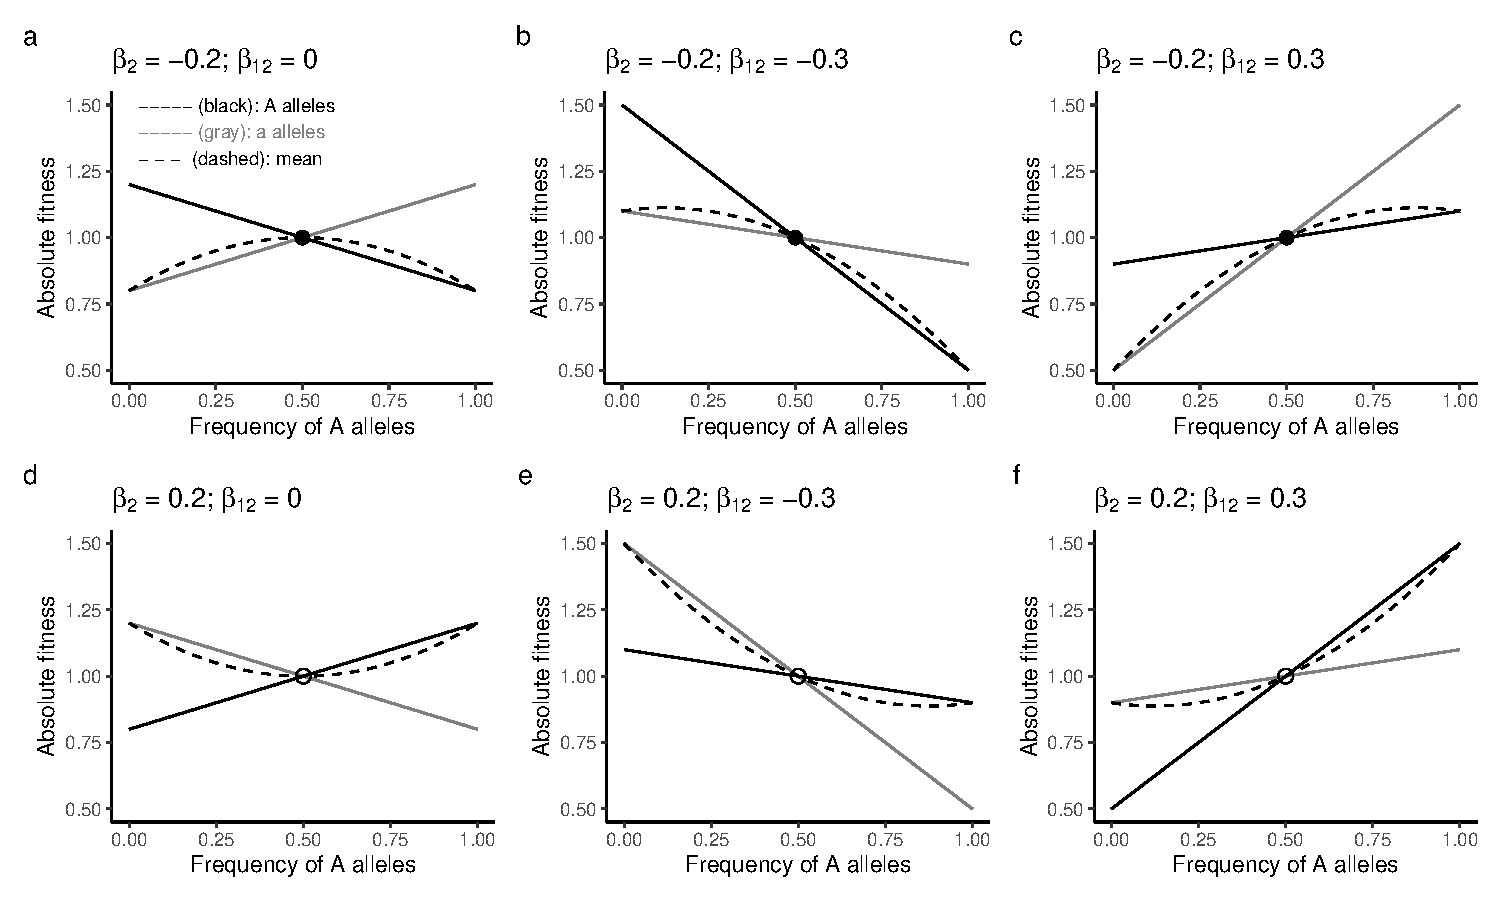
\includegraphics[width=0.7\linewidth]{AsymFDSinbred.pdf}
  \caption{Numerical examples of fitness values $y_i$ in response to allele frequency when only the AA and aa genotypes exist without mating [Equations (\ref{eq:s14a}) and (\ref{eq:s14b}) in Appendix S3]. Black and gray lines indicate the fitness functions for the AA and aa genotypes, respectively. The dashed curves indicate the mean fitness per population; that is, Equation (\ref{eq:s15}) in Appendix S3. (a) Symmetric negative frequency-dependent selection (FDS); (b) symmetric positive FDS; (c and e) asymmetric negative FDS; and (d and f) asymmetric positive FDS. Closed and open circles indicate a stable or unstable state, respectively. The base fitness and no directional selection were set at $\beta_0=1.0$ and $\beta_1=0.0$ for all panels.}
  \label{figS3:FDSinbred}
\end{figure}

\newpage
\subsection*{Supplementary Tables S3-S4 (see SuppTablesS3-S4.xlsx)}

\medskip
\noindent
\begin{table}[ht]
\caption{List of plant accessions used for genome-wide association studies (GWAS) and their phenotypes.}
    \label{tableS3:GWASdata}
\end{table}

\medskip
\noindent
\begin{table}[ht]
\caption{List of candidate genes related to self-genotype effects (a), genotype similarity effects (b), and asymmetric effects (c) on the branch number in \textit{Arabidopsis thaliana}.}
    \label{tableS4:GWAScandidates}
\end{table}


\newpage
\subsection*{Supplementary Figures S4--S10}

\begin{figure}[ht]
  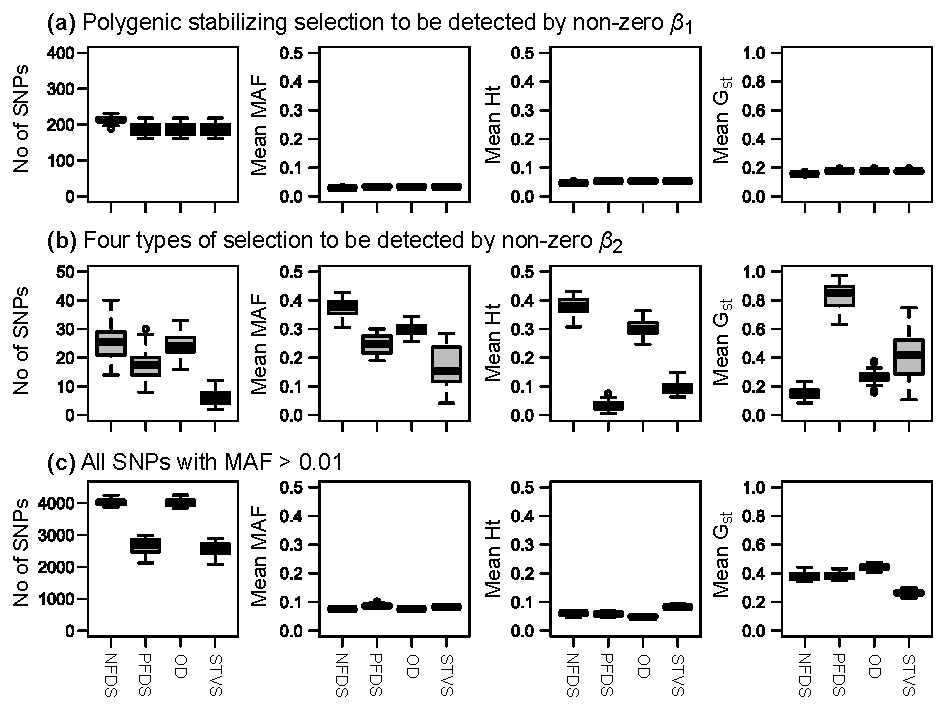
\includegraphics[width=\linewidth]{SimGenomeSummary.pdf}
  \caption{Structure of simulated genomes regarding the loci responsible for stabilizing selection (a), the other forms of selection (b), and genome-wide single nucleotide polymorphisms [SNPs](c). Number of SNPs, mean minor allele frequency (MAF), mean heterozygosity (\textit{H}\textsubscript{t}), and mean fixation indices (\textit{G}\textsubscript{st}) are shown among 30 iterations for four scenarios of selection: NFDS, negative frequency-dependent selection; PFDS, positive frequency-dependent selection; OD, overdominance; STVS, spatiotemporally varying selection.}
  \label{figS4:GenStr}
\end{figure}


\begin{figure}[]
  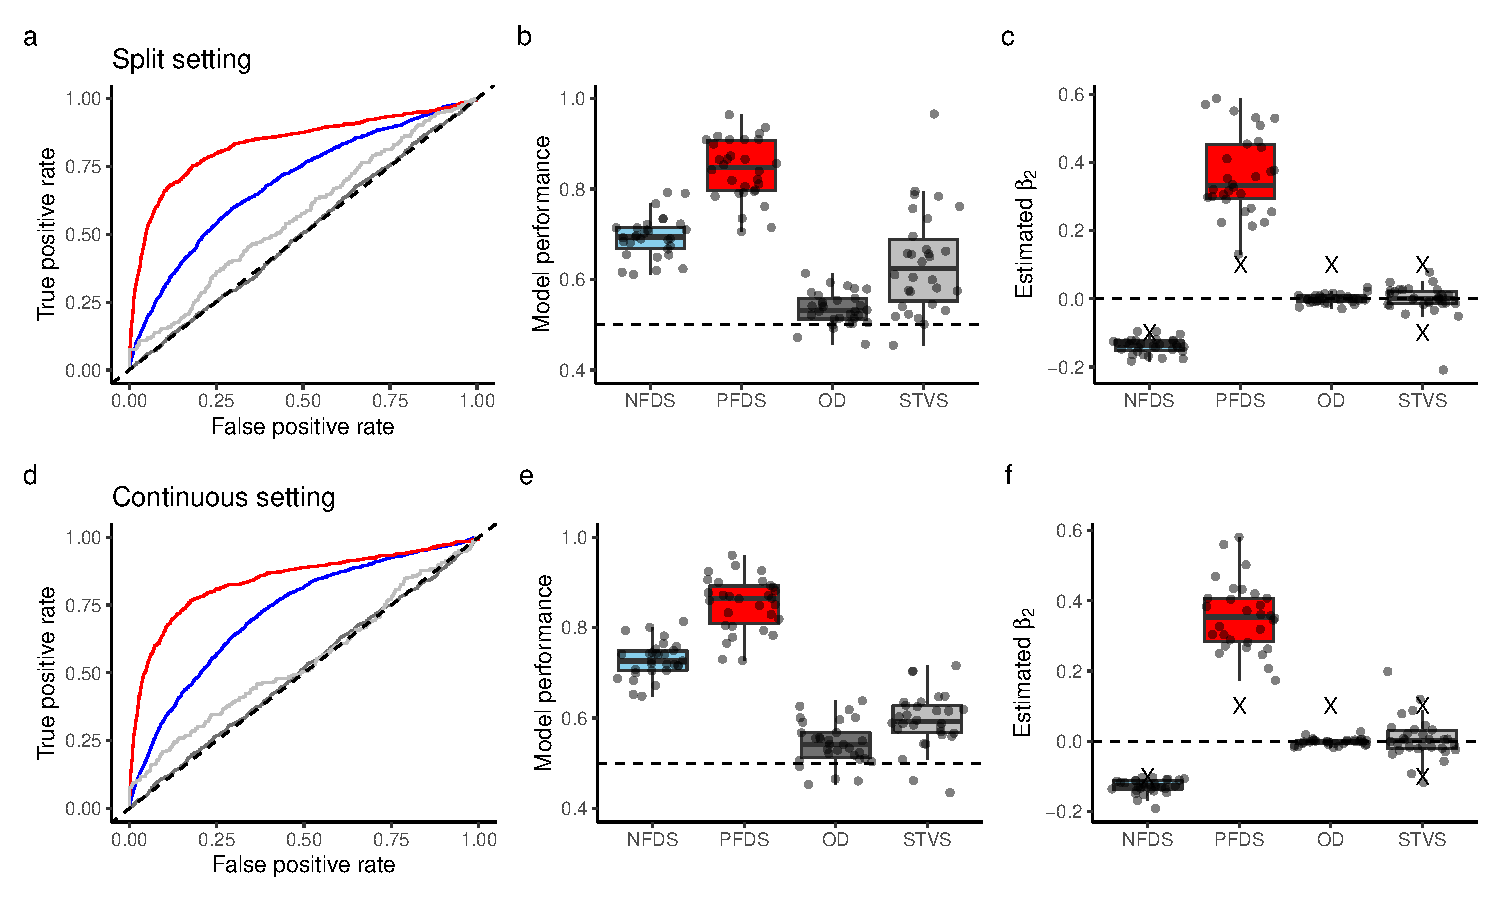
\includegraphics[width=\linewidth]{beta2LMdomi.pdf}
  \caption{Performance of standard linear models to estimate four types of simulated selection: NFDS, negative frequency-dependent selection; PFDS, positive frequency-dependent selection; OD, overdominance; and STVS, spatiotemporally varying selection. The upper and lower panels show the results of the split and continuous settings, respectively (Fig. \ref{fig1:scheme}a). The left panels show the receiver operating characteristic (ROC) curve, which indicates the relationship between the true positive rate and false positive rate. Line colors indicate different simulation scenarios (blue, NFDS; red, PFDS; black, OD; gray, STVS). The middle panel shows the area under the ROC curve (AUC). Dashed lines at AUC = 0.5, indicate no power to detect causal single nucleotide polymorphisms (SNPs). The right panels show the estimated $\beta_2$ of causal SNPs, where negative and positive values indicate negative and positive FDS, respectively. Cross marks indicate the true simulated magnitude of $\beta_2$.}
  \label{figS5:beta2LM}
\end{figure}


\begin{figure}[]
  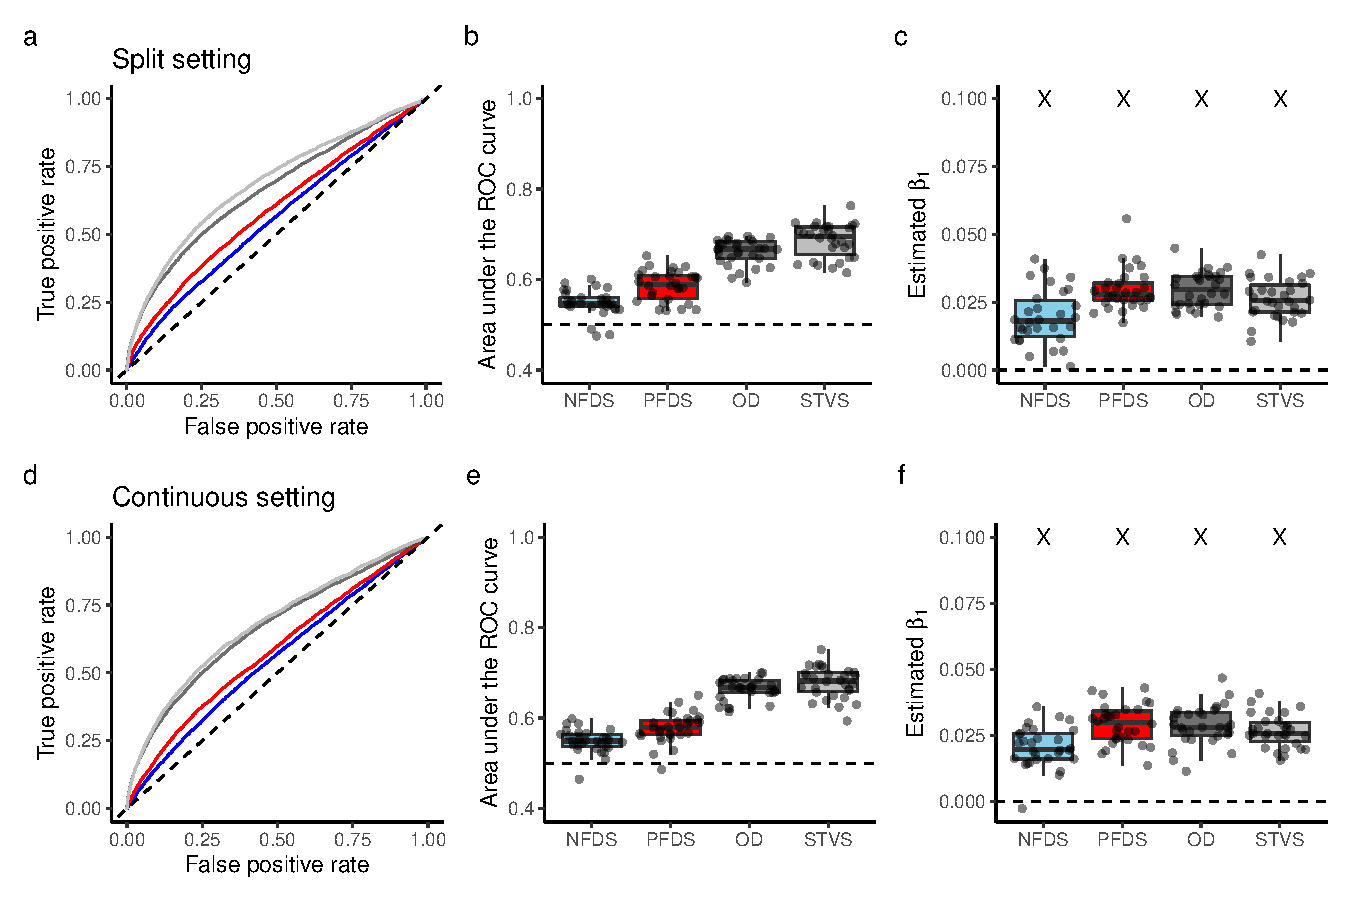
\includegraphics[width=\linewidth]{beta1LMMdomi.pdf}
  \caption{Performance of linear mixed models to detect stabilizing selection under its joint action with four types of selection: NFDS, negative frequency-dependent selection (blue); PFDS, positive frequency-dependent selection (red); OD, overdominance (dark gray); and STVS, spatiotemporally varying selection (light gray). The upper and lower panels show the results of the split and continuous settings, respectively (Fig. \ref{fig1:scheme}a). The left panels show the receiver operating characteristic (ROC) curve, which indicates the relationship between the true positive rate and false positive rate. The middle panels show the area under the ROC curve (AUC). Dashed lines at AUC = 0.5, indicate no power to detect causal single nucleotide polymorphisms (SNPs). The right panels show the estimated $\beta_1$ of causal SNPs, where negative and positive values indicate negative and positive FDS, respectively. Cross marks indicate the true simulated magnitude of $\beta_2$.}
  \label{figS6:beta1LMM}
\end{figure}


\begin{figure}[]
  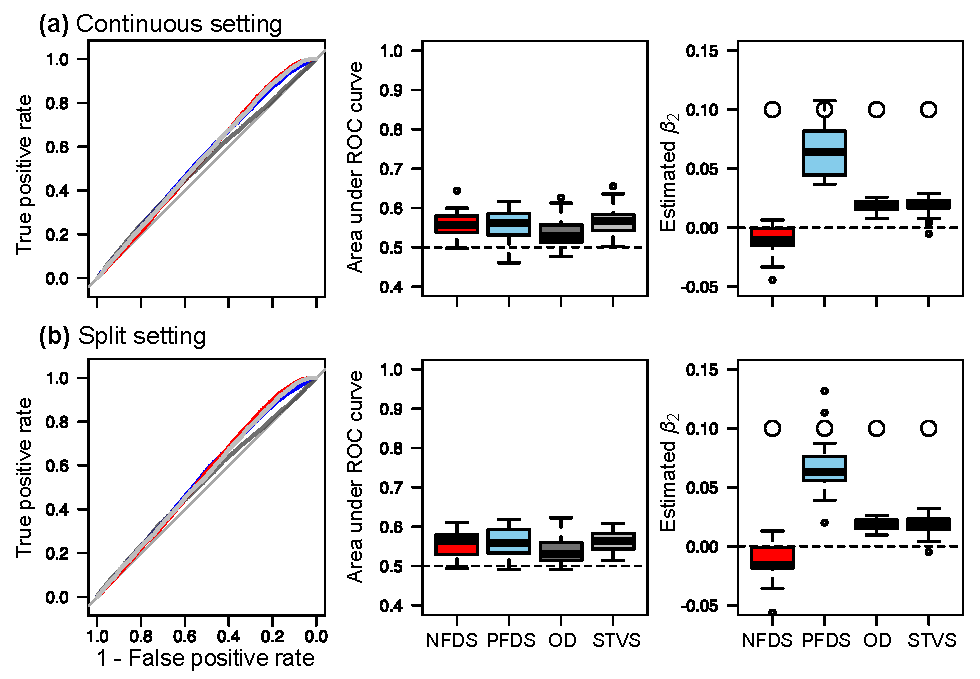
\includegraphics[width=\linewidth]{beta1LMdomi.pdf}
  \caption{Performance of standard linear models to detect stabilizing selection under its joint action with four types of selection:  NFDS, negative frequency-dependent selection (blue); PFDS, positive frequency-dependent selection (red); OD, overdominance (dark gray); and STVS, spatiotemporally varying selection (light gray). The upper and lower panels show the results of the split and continuous settings, respectively (Fig. \ref{fig1:scheme}b). The left panels show the receiver operating characteristic (ROC) curve, which indicates the relationship between the true positive rate and false positive rate. The middle panels show the area under the ROC curve (AUC). Dashed lines at AUC = 0.5, indicate no power to detect causal single nucleotide polymorphisms (SNPs). The right panels show the estimated $\beta_1$ of causal SNPs, where negative and positive values indicate negative and positive FDS, respectively. Cross marks indicate the true simulated magnitude of $\beta_2$.}
  \label{figS7:beta1LM}
\end{figure}


\begin{figure}[]
  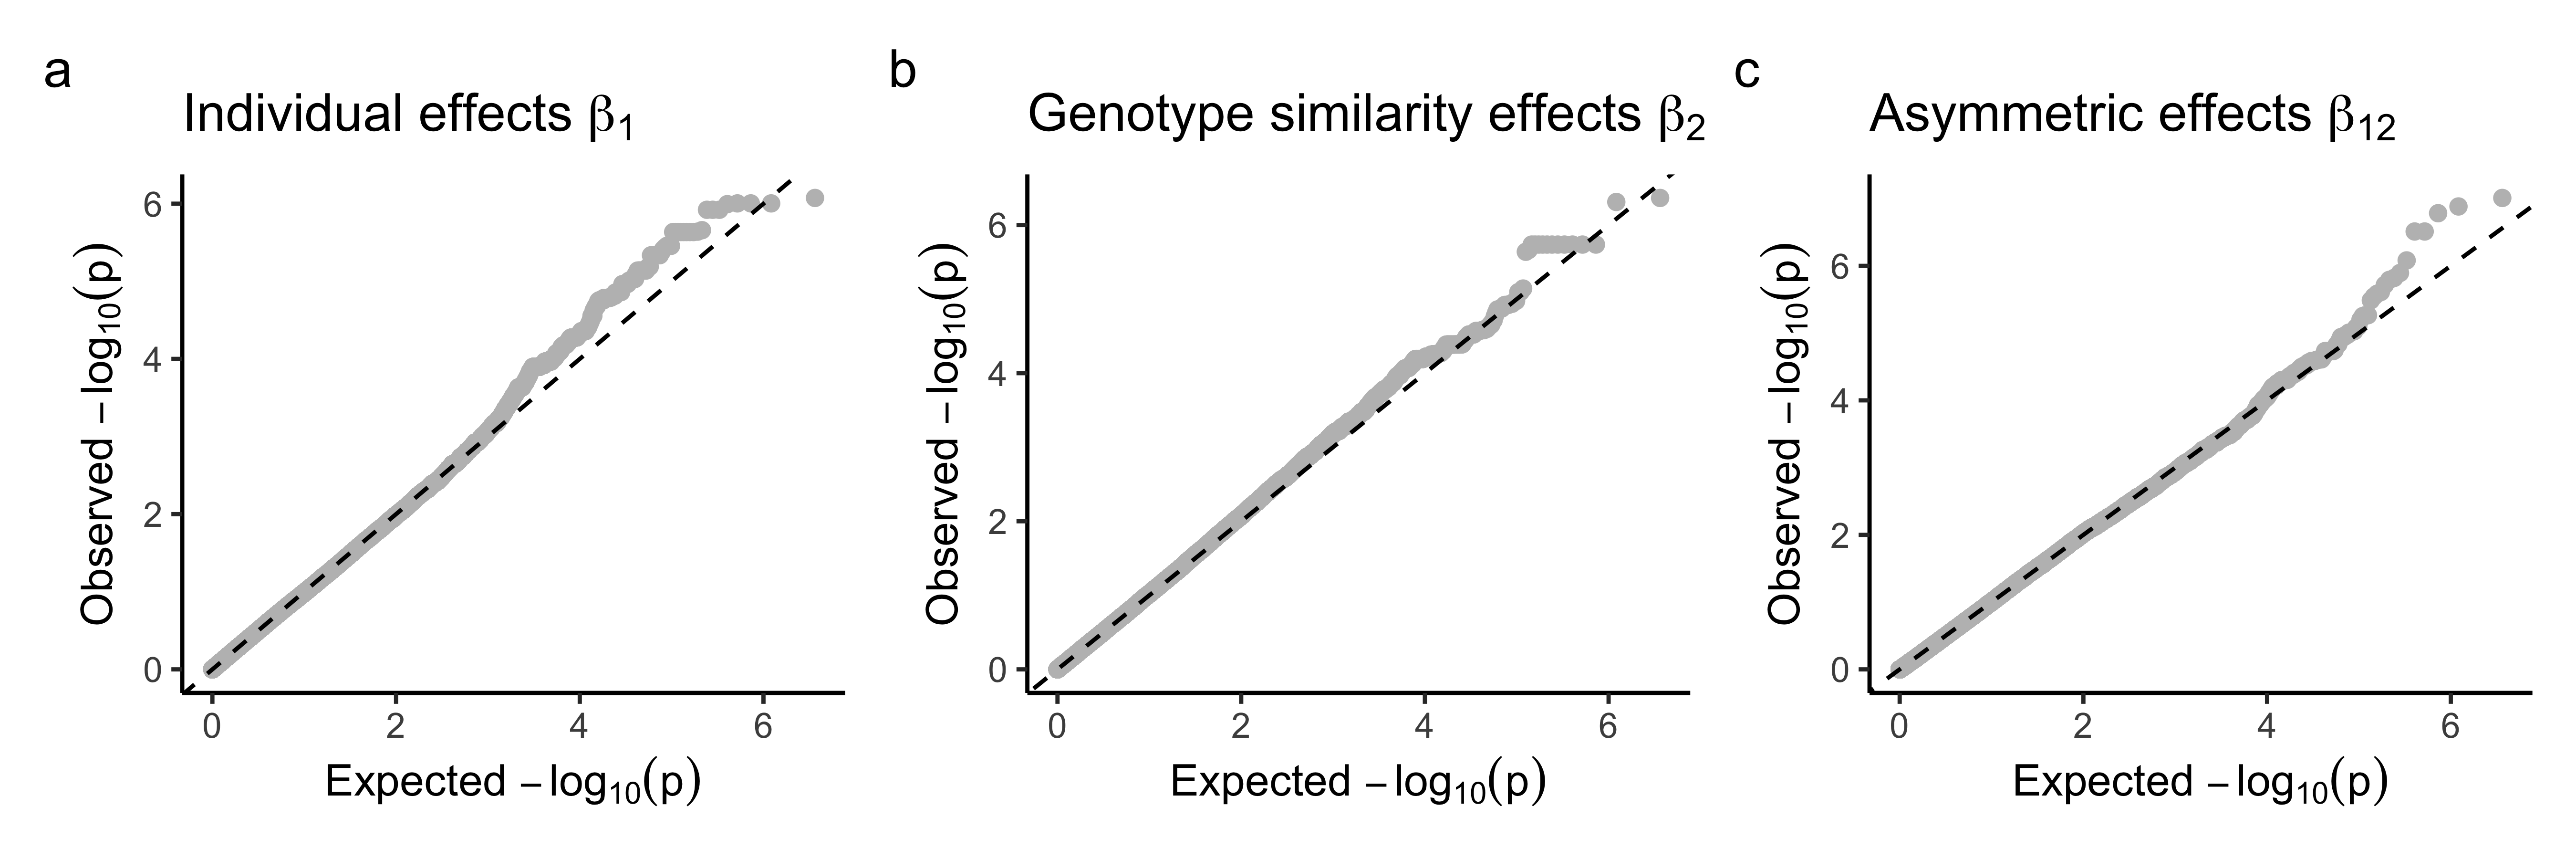
\includegraphics[width=\linewidth]{QQplotLMM.png}
  \caption{QQ-plots showing observed and expected $p$-values for the genome-wide association studies of branch number in field-grown \textit{A. thaliana}. The results for linear mixed models are shown. The left (a), middle (b), and right (c) panels display self-genotype, genotype similarity, and asymmetric effects, respectively. Dashed lines indicate the identity between the observed and expected $p$-value scores.}
  \label{figS9:QQplotLMM}
\end{figure}


\begin{figure}[]
  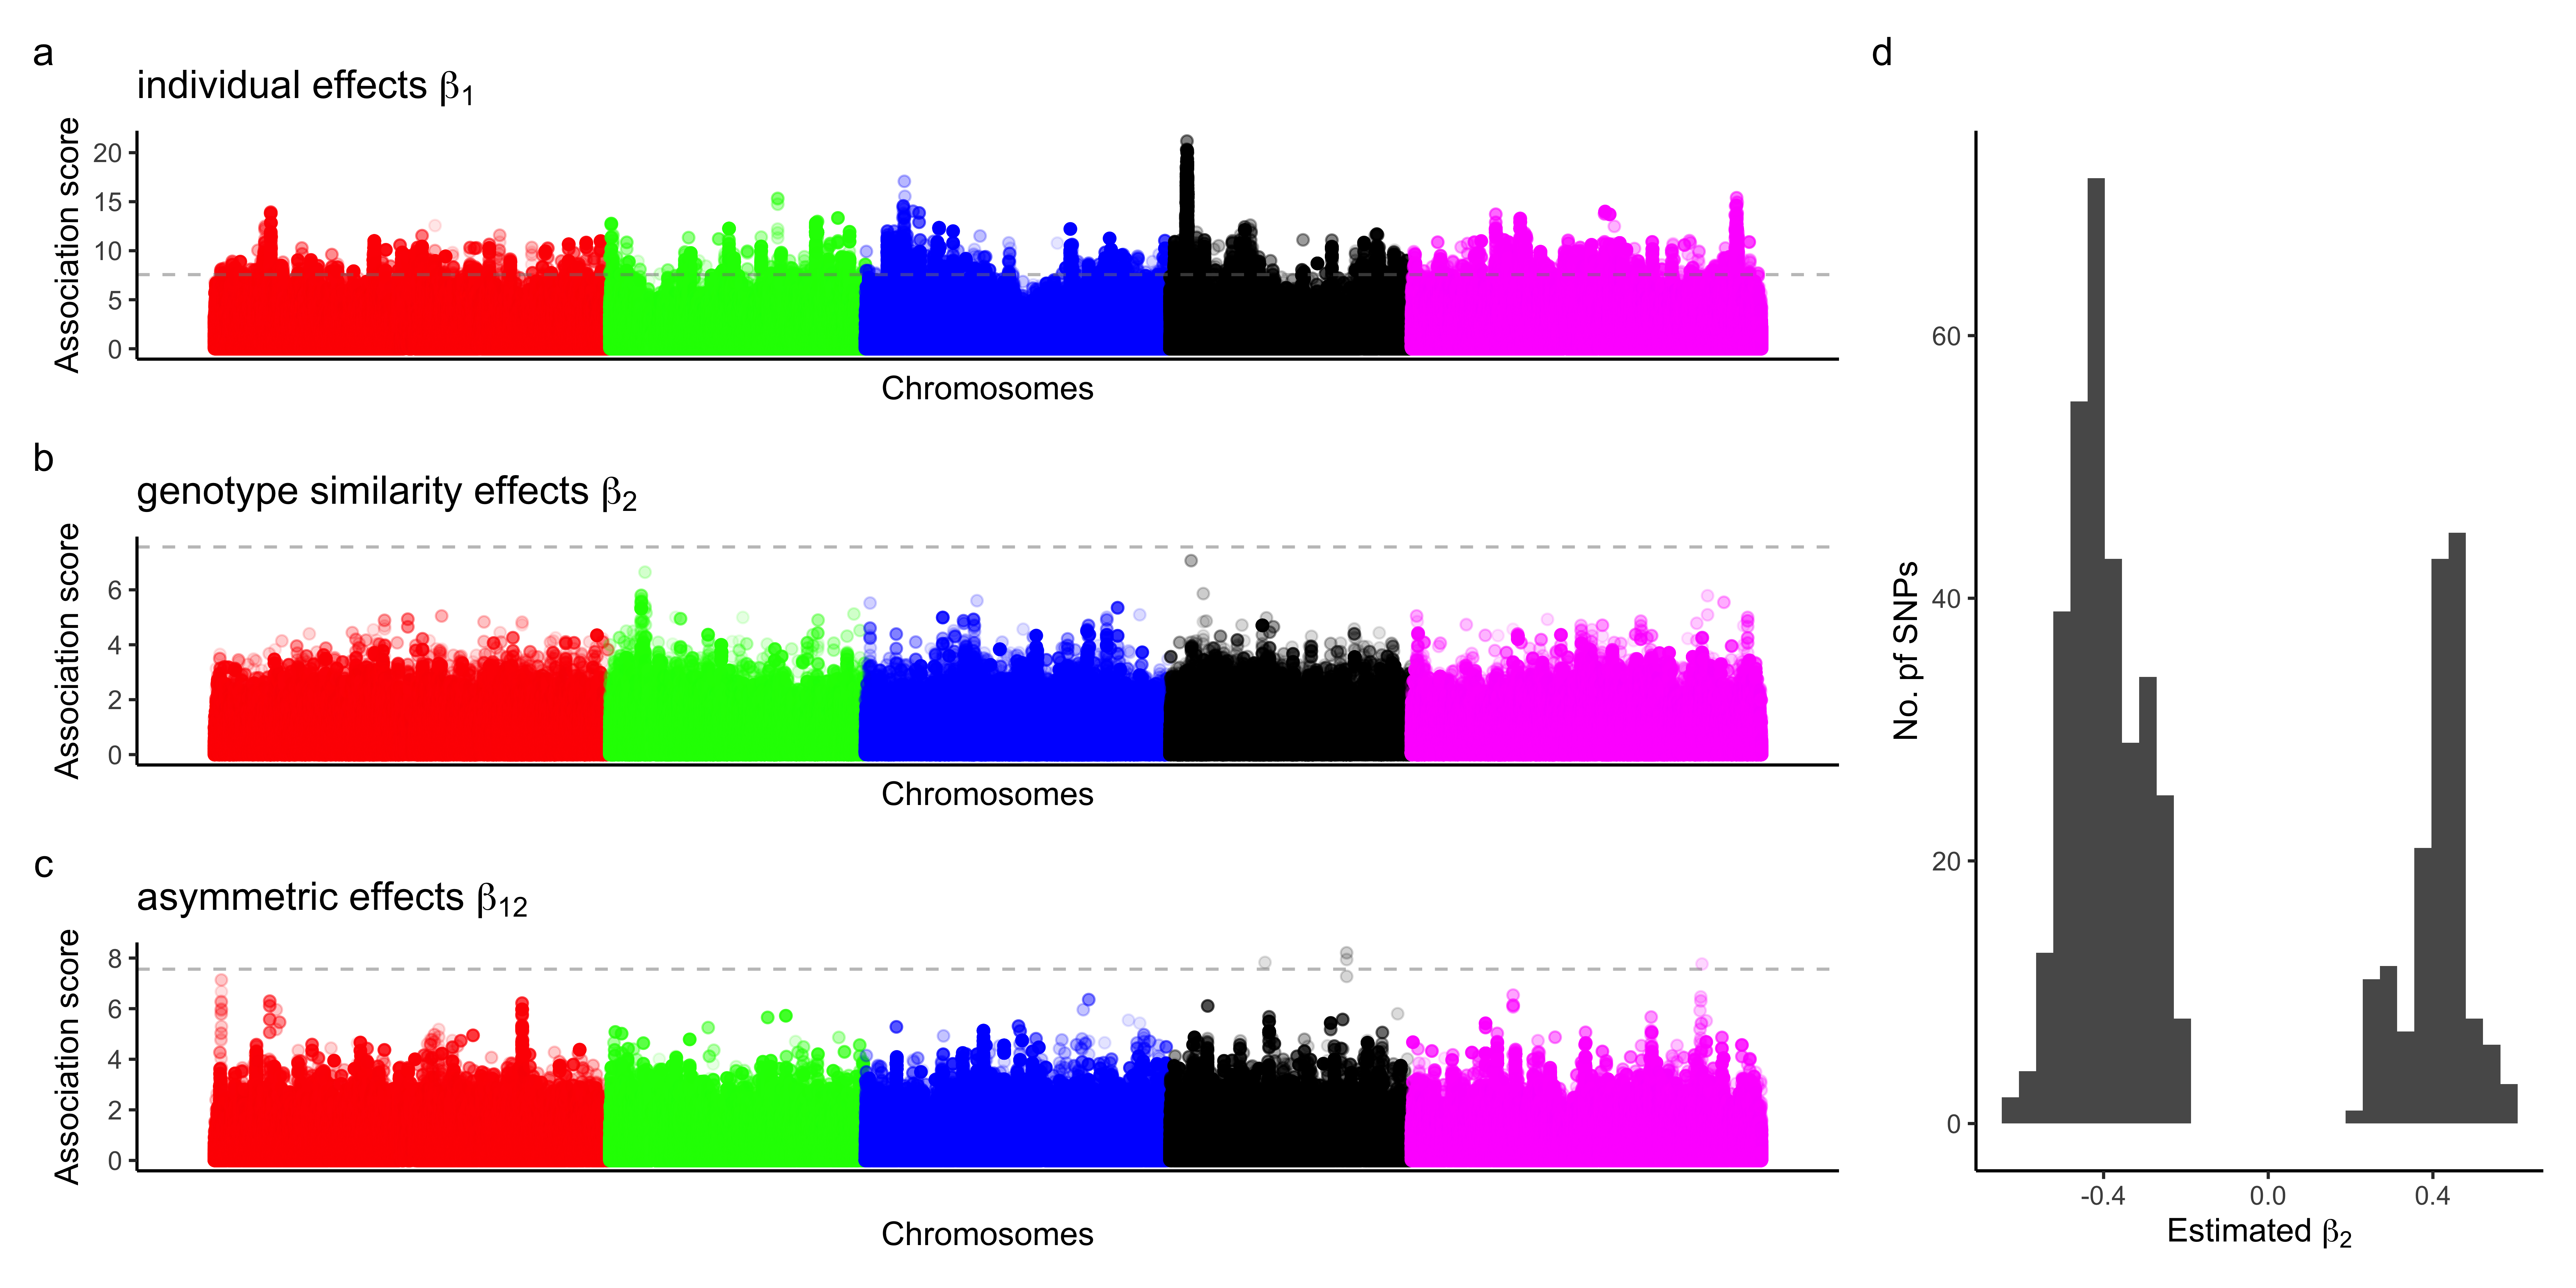
\includegraphics[width=\linewidth]{ManhattanLM.png}
  \caption{Genome-wide association studies of branch number in field-grown \textit{A. thaliana}. The results of standard linear models are presented. (a, b, and c) Manhattan plots for self-genotype effects, genotype similarity effects, and asymmetric effects, respectively. Horizontal dashed lines indicate $p$-value of $<$ 0.05, after Bonferroni correction. (d) Histogram of estimated $\beta_2$ among single nucleotide polymorphisms (SNPs) exhibiting $p$-values of $<$ 0.0001. Negative and positive $\beta_2$ infer loci responsible for negative and positive frequency-dependent selection, respectively.}
  \label{figS10:gwasLM}
\end{figure}


\begin{figure}[]
  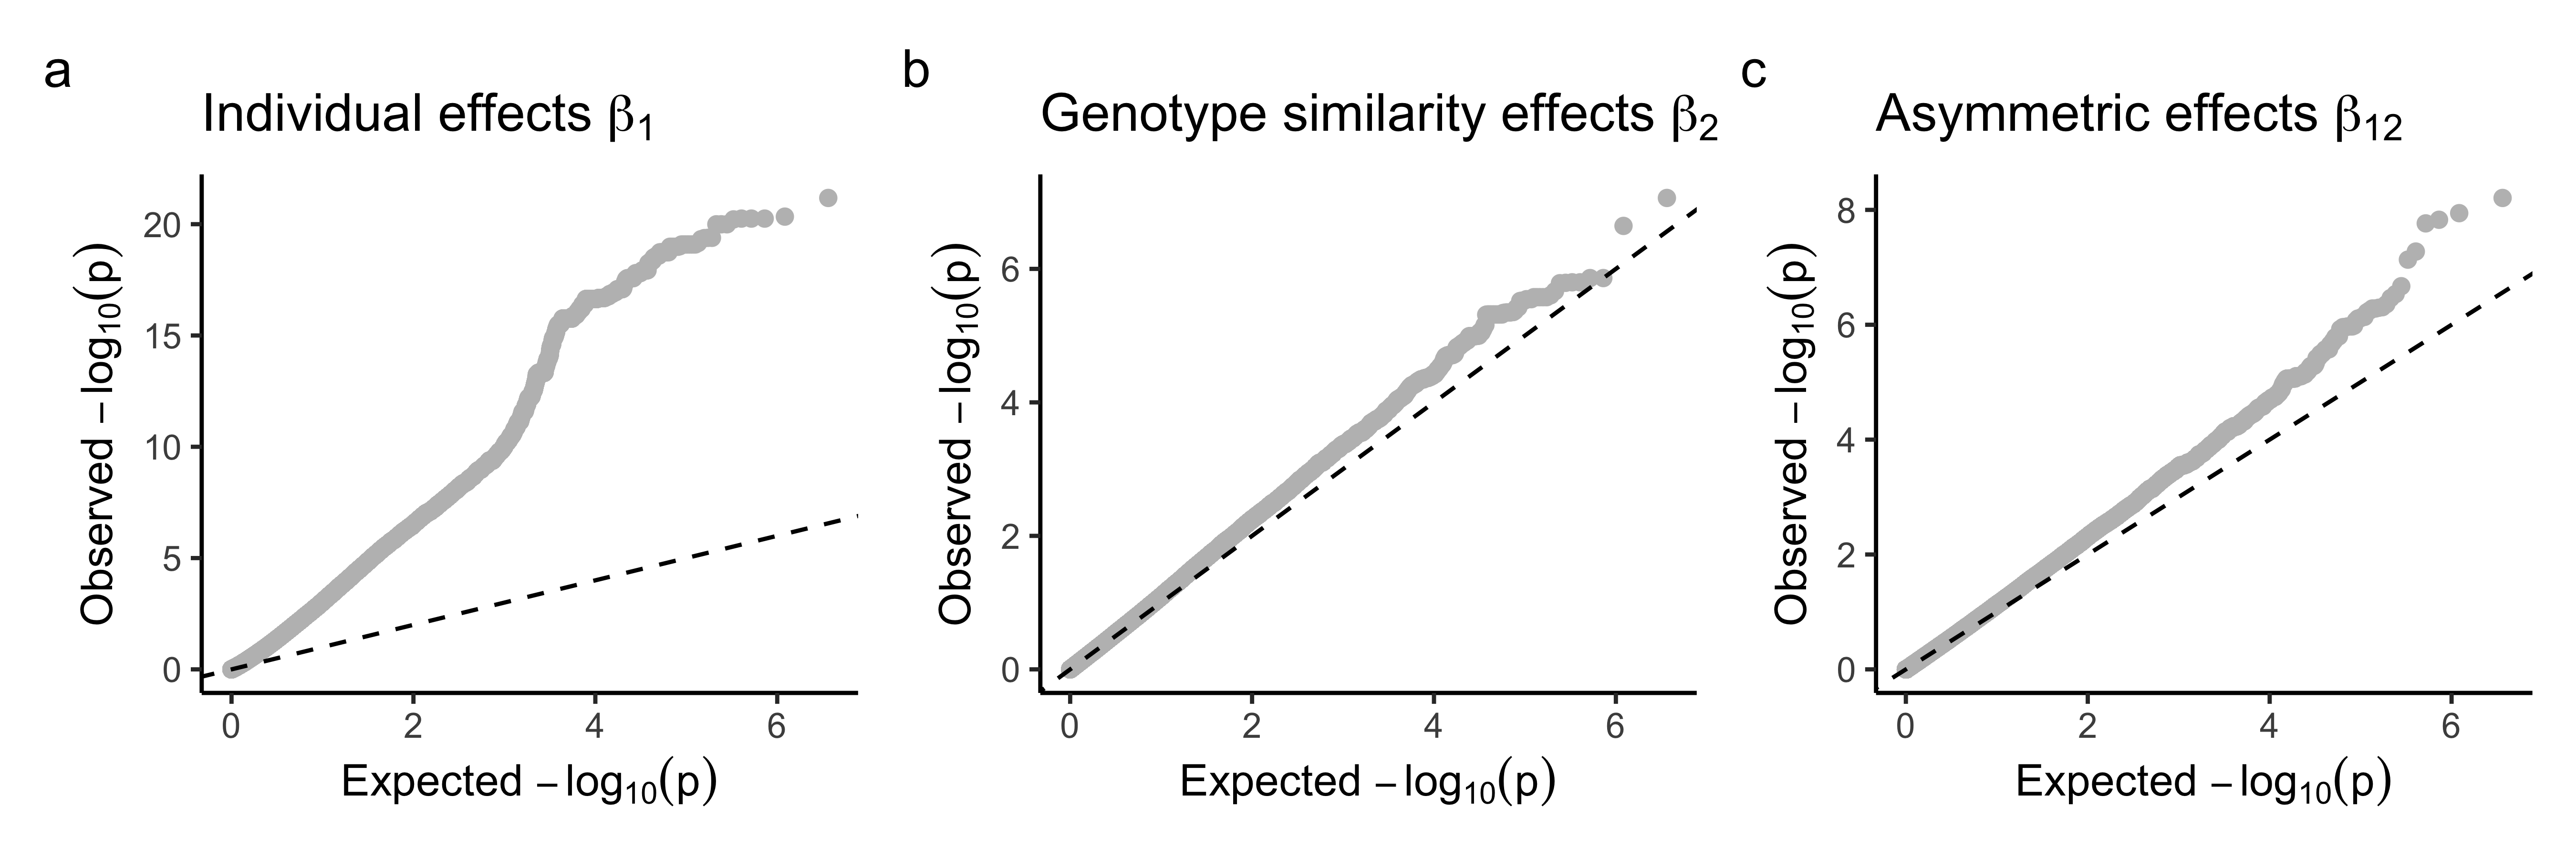
\includegraphics[width=\linewidth]{QQplotLM.png}
  \caption{QQ-plots showing observed and expected $p$-values for the genome-wide association studies of branch number in field-grown \textit{A. thaliana}. The results of standard linear models are presented. The left (a), middle (b), and right (c) panels display self-genotype, genotype similarity, and asymmetric effects, respectively. Dashed lines indicate the identity between the observed and expected $p$-value scores.}
  \label{figS11:QQplotLM}
\end{figure}


\end{document}

%%%%%%%%%%%%%%%%%%%%%%%%%%%%%%%%%%%%%%%%%%%%%%%%%%%%%%%%%%%%%%%%%%%%%%%%%%%%%%